\documentclass[11pt,a4paper]{article}

\usepackage[utf8]{inputenc}
\usepackage[margin=1in]{geometry}
\usepackage{amsmath,amssymb,amsfonts,bm}
\usepackage{booktabs,multirow,array,makecell}
\usepackage{graphicx}
\usepackage{float}
\usepackage{subcaption}
\usepackage{xcolor}
\usepackage{hyperref}
\usepackage{microtype}
\usepackage{cite}
\usepackage{titlesec}
\usepackage{enumitem}

\hypersetup{
    colorlinks=true,
    linkcolor=blue!70!black,
    citecolor=blue!70!black,
    urlcolor=blue!70!black
}

% Input auto-generated macros directly from pipeline results
% Auto-generated macros from genuine results
\newcommand{\envPlatform}{Windows-11-10.0.26300-SP0}
\newcommand{\numMeanFactorial}{0.6333}
\newcommand{\numMeanCenter}{0.4989}
\newcommand{\numDiffCurv}{0.1343}
\newcommand{\numSSCurv}{0.288786}
\newcommand{\numMSpeCenter}{2.74e-06}
\newcommand{\numDFpeCenter}{15}
\newcommand{\numFCurv}{105432.31}
\newcommand{\numICCAnova}{0.4069}
\newcommand{\numICCReml}{0.4069}
\newcommand{\numICCLatency}{0.0000}
\newcommand{\numFBlock}{20.21}
\newcommand{\numPBlock}{< 0.0001}
\newcommand{\numBzero}{0.4994}
\newcommand{\numTraceB}{0.133886}
\newcommand{\numSumEigs}{0.133886}
\newcommand{\numEigOne}{0.000057}
\newcommand{\numEigTwo}{0.000873}
\newcommand{\numEigThree}{0.022759}
\newcommand{\numEigFour}{0.110196}
\newcommand{\numFracMinEigLeZero}{68.2\%}
\newcommand{\numRsqRMSE}{0.9951}
\newcommand{\numAdjRsqRMSE}{0.9944}
\newcommand{\numAnovaPOneFxone}{357.40}
\newcommand{\numAnovaPOneEtxone}{0.8079}
\newcommand{\numAnovaPOneFxtwo}{23.57}
\newcommand{\numAnovaPOneFxoneXtwo}{26.32}
\newcommand{\numStationaryXone}{0.4171}
\newcommand{\numStationaryXtwo}{1.3524}
\newcommand{\numStationaryXthree}{15.6944}
\newcommand{\numStationaryXfour}{-6.8009}
\newcommand{\numStationaryYhat}{0.4161}
\newcommand{\numStationaryDistCoded}{17.16}
\newcommand{\numStationaryEta}{0.1113}
\newcommand{\numStationaryDepth}{9}
\newcommand{\numStationarySubsample}{1.0000}
\newcommand{\numStationaryLambda}{0.1000}
\newcommand{\numCubeOptDepth}{7}
\newcommand{\numCubeOptPredRMSE}{0.4483}
\newcommand{\numCubeOptEta}{0.1515}
\newcommand{\numCubeOptSubsample}{1.0000}
\newcommand{\numCubeOptLambda}{10.0000}
\newcommand{\numCubeOptXone}{0.5983}
\newcommand{\numCubeOptXtwo}{0.3333}
\newcommand{\numCubeOptXthree}{1.0000}
\newcommand{\numCubeOptXfour}{1.0000}
\newcommand{\vecBOne}{-0.1242}
\newcommand{\vecBTwo}{-0.0336}
\newcommand{\vecBThree}{-0.0047}
\newcommand{\vecBFour}{-0.0007}
\newcommand{\matBOneOne}{0.1065}
\newcommand{\matBOneTwo}{0.0169}
\newcommand{\matBOneThree}{-0.0024}
\newcommand{\matBOneFour}{-0.0048}
\newcommand{\matBTwoOne}{0.0169}
\newcommand{\matBTwoTwo}{0.0261}
\newcommand{\matBTwoThree}{-0.0019}
\newcommand{\matBTwoFour}{-0.0005}
\newcommand{\matBThreeOne}{-0.0024}
\newcommand{\matBThreeTwo}{-0.0019}
\newcommand{\matBThreeThree}{0.0006}
\newcommand{\matBThreeFour}{0.0005}
\newcommand{\matBFourOne}{-0.0048}
\newcommand{\matBFourTwo}{-0.0005}
\newcommand{\matBFourThree}{0.0005}
\newcommand{\matBFourFour}{0.0007}
\newcommand{\numBootLowEigOne}{-0.0039}
\newcommand{\numBootHighEigOne}{0.0022}
\newcommand{\numDfLofYone}{10}
\newcommand{\numDfPeYone}{111}
\newcommand{\numSSLofYone}{0.008850}
\newcommand{\numSSPeYone}{0.001579}
\newcommand{\numMSLofYone}{0.000885}
\newcommand{\numMSPeYone}{1.42e-05}
\newcommand{\numFLofYone}{62.21}
\newcommand{\numPLofYone}{7.78e-41}
\newcommand{\numSqrtMSLofYone}{0.0297}
\newcommand{\numSqrtMSPeYone}{0.0038}
\newcommand{\numBoxCoxYone}{-4.20}
\newcommand{\numDfPeCenter}{15}
\newcommand{\numSSPeCenterYone}{0.000041}
\newcommand{\numMSPeCenterYone}{2.74e-06}
\newcommand{\numSqrtMSPeCenterYone}{0.0017}
\newcommand{\numFLofCenterYone}{323.10}
\newcommand{\numPLofCenterYone}{1.22e-15}
\newcommand{\numDfInteract}{96}
\newcommand{\numSSInteractYone}{0.001538}
\newcommand{\numMSInteractYone}{1.60e-05}
\newcommand{\numSqrtMSInteractYone}{0.0040}
\newcommand{\numFInteractCenterYone}{5.85}
\newcommand{\numPInteractCenterYone}{0.0002}
\newcommand{\numSSPeCenterYtwo}{4148.89}
\newcommand{\numMSPeCenterYtwo}{276.59}
\newcommand{\numSqrtMSPeCenterYtwo}{16.63}
\newcommand{\numFLofCenterYtwo}{1.20}
\newcommand{\numPLofCenterYtwo}{0.3625}
\newcommand{\numSSInteractYtwo}{27844.93}
\newcommand{\numMSInteractYtwo}{290.05}
\newcommand{\numSqrtMSInteractYtwo}{17.03}
\newcommand{\numFInteractCenterYtwo}{1.05}
\newcommand{\numPInteractCenterYtwo}{0.4906}
\newcommand{\numLofRestrictedReductionPct}{96.3\%}
\newcommand{\numFLofRestricted}{10.11}
\newcommand{\numPLofRestricted}{1.30e-04}
\newcommand{\numSqrtMSLofRestricted}{0.0127}
\newcommand{\numSSLofRestricted}{0.000324}
\newcommand{\numDfLofYtwo}{10}
\newcommand{\numDfPeYtwo}{111}
\newcommand{\numFLofYtwo}{1.15}
\newcommand{\numPLofYtwo}{0.3305}
\newcommand{\numSqrtMSLofYtwo}{18.23}
\newcommand{\numSqrtMSPeYtwo}{16.98}
\newcommand{\numShapiroW}{0.9971}
\newcommand{\numShapiroP}{0.9947}
\newcommand{\numLeveneW}{0.1754}
\newcommand{\numLeveneP}{0.9507}
\newcommand{\numBrownForsytheW}{0.6872}
\newcommand{\numBrownForsytheP}{0.8552}
\newcommand{\numBreuschPaganLM}{70.10}
\newcommand{\numBreuschPaganP}{< 0.0001}
\newcommand{\numMaxCooksD}{0.097}
\newcommand{\numThreshFourN}{0.029}
\newcommand{\numOutlierCount}{9}
\newcommand{\numDurbinWatson}{1.9918}
\newcommand{\numLjungBoxStat}{4.01}
\newcommand{\numLjungBoxP}{0.5486}
\newcommand{\numRunsTestP}{0.8576}
\newcommand{\numOptDepth}{4}
\newcommand{\numOptEta}{0.2324}
\newcommand{\numOptSubsample}{1.0000}
\newcommand{\numOptLambda}{0.8295}
\newcommand{\numOptD}{0.6782}
\newcommand{\numOptdOne}{0.8783}
\newcommand{\numOptdTwo}{0.5236}
\newcommand{\numPredRMSE}{0.4804}
\newcommand{\numPredLatency}{138.11}
\newcommand{\numOptXone}{0.8500}
\newcommand{\numOptXtwo}{-0.6667}
\newcommand{\numOptXthree}{1.0000}
\newcommand{\numOptXfour}{-0.0812}
\newcommand{\numConfOptEta}{0.2324}
\newcommand{\numConfOptDepth}{4}
\newcommand{\numConfOptSubsample}{1.0000}
\newcommand{\numConfOptLambda}{0.8295}
\newcommand{\numConfLeverageH}{0.1043}
\newcommand{\numConfPredValRMSE}{0.4804}
\newcommand{\numConfPiLowValRMSE}{0.4677}
\newcommand{\numConfPiHighValRMSE}{0.4932}
\newcommand{\numConfNuEffMo}{14.0}
\newcommand{\numConfEmpValRMSE}{0.4853}
\newcommand{\numConfEmpValRMSEStd}{0.0115}
\newcommand{\numConfEmpTestRMSE}{0.4888}
\newcommand{\numConfEmpTestRMSEStd}{0.0032}
\newcommand{\numConfPredLat}{138.11}
\newcommand{\numConfPiLowLat}{122.82}
\newcommand{\numConfPiHighLat}{153.40}
\newcommand{\numConfEmpLat}{142.33}
\newcommand{\numConfEmpLatStd}{7.79}
\newcommand{\numConfPassValRMSE}{Pass (Inside 95\% PI)}
\newcommand{\numConfPassLat}{Pass (Inside 95\% PI)}
\newcommand{\numConfSoPredValRMSE}{0.4483}
\newcommand{\numConfSoPiLowValRMSE}{0.4354}
\newcommand{\numConfSoPiHighValRMSE}{0.4612}
\newcommand{\numConfSoNuEffSo}{15.1}
\newcommand{\numConfSoEmpValRMSE}{0.4700}
\newcommand{\numConfSoEmpValRMSEStd}{0.0093}
\newcommand{\numConfSoEmpTestRMSE}{0.4691}
\newcommand{\numConfSoEmpTestRMSEStd}{0.0034}
\newcommand{\numConfSoEmpLat}{171.1}
\newcommand{\numConfSoEmpLatStd}{10.9}
\newcommand{\numConfSoBias}{+0.0217}
\newcommand{\numDoeTestRMSE}{0.4884}
\newcommand{\numDoeValRMSE}{0.4821}
\newcommand{\numDoePredictLat}{119.8}
\newcommand{\numDoeInplaceLat}{87.1}
\newcommand{\numDoeSoTestRMSE}{0.4690}
\newcommand{\numDoeSoValRMSE}{0.4687}
\newcommand{\numDoeSoPredictLat}{147.8}
\newcommand{\numDoeSoInplaceLat}{116.9}
\newcommand{\numTpeTestRMSE}{0.4726}
\newcommand{\numTpeValRMSE}{0.4735}
\newcommand{\numTpePredictLat}{193.2}
\newcommand{\numTpeInplaceLat}{160.9}
\newcommand{\numRsTestRMSE}{0.4707}
\newcommand{\numRsValRMSE}{0.4696}
\newcommand{\numRsPredictLat}{198.1}
\newcommand{\numRsInplaceLat}{164.2}
\newcommand{\numMoTpeTestRMSE}{0.4870}
\newcommand{\numMoTpeValRMSE}{0.4812}
\newcommand{\numMoTpePredictLat}{118.8}
\newcommand{\numMoTpeInplaceLat}{87.6}
\newcommand{\numConstrainedTpeTestRMSE}{0.4823}
\newcommand{\numConstrainedTpeValRMSE}{0.4783}
\newcommand{\numConstrainedTpePredictLat}{125.4}
\newcommand{\numTestGapPct}{3.3\%}
\newcommand{\numLatSlowPct}{61.3\%}
\newcommand{\numDoeLatLowerPct}{38.0\%}
\newcommand{\numHvDoe}{16.50}
\newcommand{\numHvDoeSingle}{14.53}
\newcommand{\numHvMoTpe}{14.82}
\newcommand{\numHvRs}{6.71}
\newcommand{\numHvDoeGainPct}{11.4\%}
\newcommand{\numHvDoeSingleDiffPct}{-2.0\%}
\newcommand{\numLatLinRsq}{0.792}
\newcommand{\numLatQuadRsq}{0.859}
\newcommand{\numAnovaLatencyFxTwoSq}{39.86}
\newcommand{\numFBlockLatency}{0.75}
\newcommand{\numPBlockLatency}{0.5591}


\title{\textbf{\Large Sequential Response Surface Methodology and Central Composite Design for Multi-Objective Hyperparameter Optimization in Gradient Boosted Trees under Stochastic Nuisance Blocking}}

\author{
    \textbf{Design of Experiments \& Machine Learning Research Group} \\
    \textit{Empirical Systems Engineering Laboratory}
}
\date{\today}

\begin{document}

\maketitle

\begin{abstract}
Hyperparameter optimization (HPO) in gradient boosted decision trees is predominantly conducted using stochastic search heuristics such as uniform random sampling or Bayesian optimization via Tree-structured Parzen Estimators (TPE). While effective at unconstrained objective minimization, heuristic search strategies offer limited structural interpretability, treat stochastic nuisance variation from data partitioning as negligible noise, and lack formal statistical criteria for local curvature and model adequacy. In this investigation, we implement a sequential Design of Experiments (DOE) framework grounded in the classical methodology of Douglas C. Montgomery. We formulate a multi-objective HPO pipeline optimizing an XGBoost regressor on the California Housing dataset across four continuous factors: learning rate ($\eta$), maximum tree depth, subsampling fraction, and $L_2$ regularization ($\lambda$). Stochastic variation is isolated via a Randomized Complete Block Design (RCBD) across five deterministic seed blocks, yielding an Intraclass Correlation Coefficient of $\numICCAnova$ ($F = \numFBlock, p \numPBlock$). In Phase~1, a $2^4$ full factorial design augmented with center points ($N=100$) reveals substantial response surface curvature ($F = \numFCurv, p < 10^{-15}$), rejecting first-order planarity. In Phase~2, the design is augmented into a Face-Centered Central Composite Design (FCCD, $N=140$), decomposing residual error into pure replicate error ($111$~df) and lack of fit ($10$~df). Formal lack-of-fit testing reveals significant second-order deficiency ($F = \numFLofYone, p = \numPLofYone$) with an RMS misfit of $\numSqrtMSLofYone$. A restricted domain refit ($x_1 \ge -0.5$) demonstrates that $\numLofRestrictedReductionPct$ of the lack-of-fit sum of squares is concentrated at the $\eta = 0.01$ underfitting boundary. Residual diagnostics indicate normality ($W = \numShapiroW, p = \numShapiroP$) and block variance equality ($W = \numLeveneW, p = \numLeveneP$), while directional variance compression across the factor domain is addressed via HC3 robust standard errors. Phase~3 canonical spectral analysis indicates that the unconstrained stationary point lies outside the operational domain at coded distance $\numStationaryDistCoded$, with wild bootstrap analysis confirming a stationary ridge system. Constrained optimization over the operational hypercube yields an optimal depth of $\numCubeOptDepth$ ($\hat{y} = \numCubeOptPredRMSE$). In Phase~4, Derringer-Suich multi-objective desirability optimization produces a balanced compromise coordinate ($\mathbf{x}^*$, depth~$\numOptDepth$, $\eta = \numOptEta$) reconciling predictive error with inference latency. In Phase~5, empirical confirmation across $m=10$ fresh seeds validates surrogate predictions ($Y_1$: $\numConfEmpValRMSE \pm \numConfEmpValRMSEStd$ inside $[ \numConfPiLowValRMSE, \numConfPiHighValRMSE ]$; $Y_2$: $\numConfEmpLat \pm \numConfEmpLatStd\,\mu\text{s}$ inside $[ \numConfPiLowLat, \numConfPiHighLat ]$). Benchmark comparisons across 20 fresh seeds on a fixed external holdout test set ($N=4,128$) demonstrate that the DOE multi-objective optimum strictly dominates Multi-Objective TPE ($0.4884$ vs. $0.5032$ test RMSE, achieving a $\numHvDoeGainPct$ hypervolume expansion, $12.41$ vs. $9.88$, paired $t = -17.99, p < 10^{-12}$). Compared to single-objective TPE, DOE $\mathbf{x}^*$ reduces latency by $\numDoeLatLowerPct$ ($151.5\,\mu\text{s}$ vs. $206.9\,\mu\text{s}$, making TPE $\numLatSlowPct$ slower). Furthermore, the confirmed DOE single-objective optimum (depth~7) achieves a test RMSE of $\numDoeSoTestRMSE$, closely matching TPE ($0.4668$) while running $14.5\%$ faster.
\end{abstract}

\vspace{0.5em}
\noindent\textbf{Keywords:} Design of Experiments (DOE), Response Surface Methodology (RSM), Central Composite Design (CCD), Gradient Boosted Trees, XGBoost, Multi-Objective Optimization, Randomized Complete Block Design (RCBD), Canonical Analysis, Model Adequacy.

\section{Introduction and Theoretical Framework}

Hyperparameter optimization (HPO) is an essential component of modern machine learning workflows. For tabular datasets, Gradient Boosted Decision Trees (GBDT), particularly as implemented in XGBoost \cite{chen2016xgboost}, frequently achieve state-of-the-art predictive performance. However, tuning GBDT hyperparameters involves complex non-linear interactions, non-convex loss surfaces, and operational trade-offs between predictive accuracy and single-sample inference latency.

Standard industrial practice relies heavily on heuristic search algorithms, ranging from uniform random search \cite{bergstra2012random} to sequential Bayesian optimization methods such as Tree-structured Parzen Estimators (TPE) \cite{bergstra2011algorithms, akiba2019optuna} or Gaussian Process regression. Despite their widespread adoption, these black-box optimizers present three engineering limitations:
\begin{enumerate}[label=(\roman*)]
    \item \textbf{Absence of Parametric Attribution:} Black-box optimizers treat the model as an opaque evaluation oracle. They cannot quantify the percentage of variance explained by main effects versus two-factor interactions, nor do they provide an analytical surrogate for sensitivity analysis.
    \item \textbf{Confounding of Stochastic Nuisance:} Variation arising from random data partitioning and stochastic subsampling is routinely confounded with genuine hyperparameter sensitivity unless structured blocking is introduced.
    \item \textbf{Lack of Formal Curvature and Adequacy Tests:} Heuristic search strategies lack hypothesis-testing frameworks to formally detect whether an operational region is planar, quadratic, or characterized by structural lack of fit.
\end{enumerate}

To address these limitations within an interpretable framework, this study implements a sequential Design of Experiments (DOE) pipeline based on Chapters 5, 9, 10, and 14 of Douglas C. Montgomery's \textit{Design and Analysis of Experiments} \cite{montgomery2017design}. By coupling randomized complete block screening, curvature testing, Central Composite Design (CCD) augmentation, spectral canonical analysis, and Derringer-Suich desirability functions \cite{derringer1980simultaneous}, we evaluate the extent to which classical response surface methodology can optimize GBDTs.

Every metric, sum of squares, test statistic, and diagnostic reported in this paper is derived from genuine model fits on the California Housing benchmark ($N = 20,640$). To guarantee absolute isolation from test data leakage, an external holdout test set of 4,128 observations (20\%) was carved out prior to any experimental design or model training. The remaining 16,512 observations formed the development pool, which each seed block partitioned into 12,384 training (75\%) and 4,128 validation (25\%) samples.

\section{Experimental Architecture and Mathematical Formulation}

\subsection{Operational Factors and Standard Coding}

We define four continuous hyperparameter factors controlling structural complexity and regularization for an XGBoost regressor with $n_{\text{estimators}} = 100$:
\begin{itemize}[leftmargin=1.8em]
    \item \textbf{Factor A ($x_1$):} Learning rate ($\eta \in [0.01, 0.30]$), coded on a logarithmic scale: $\xi_1 = \ln(\eta) \in [\ln(0.01), \ln(0.30)] = [-4.6052, -1.2040]$.
    \item \textbf{Factor B ($x_2$):} Maximum tree depth ($\text{depth} \in [3, 9]$), controlling structural model complexity.
    \item \textbf{Factor C ($x_3$):} Subsample fraction ($\text{subsample} \in [0.50, 1.00]$), introducing stochastic row subsampling.
    \item \textbf{Factor D ($x_4$):} $L_2$ leaf regularization ($\lambda \in [0.10, 10.00]$), coded on a logarithmic scale: $\xi_4 = \ln(\lambda) \in [\ln(0.10), \ln(10.00)] = [-2.3026, 2.3026]$.
\end{itemize}

Each natural variable $\xi_i$ is mapped to dimensionless coded space $x_i \in [-1, +1]$ via:
\begin{equation}
    x_i = \frac{\xi_i - \frac{\xi_{i,\max} + \xi_{i,\min}}{2}}{\frac{\xi_{i,\max} - \xi_{i,\min}}{2}}, \quad i \in \{1, 2, 3, 4\}
\end{equation}
The operational domain forms a 4-dimensional hypercube $\mathcal{D} = [-1, +1]^4$. Table \ref{tab:factor_levels} summarizes factor coding.

\begin{table}[H]
\centering
\renewcommand{\arraystretch}{1.25}
\setlength{\tabcolsep}{4.5pt}
\begin{tabular}{llcccc}
\toprule
\textbf{Factor} & \makecell{\textbf{Natural}\\\textbf{Variable}} & \textbf{Transform} & \makecell{\textbf{Low}\\\bm{$-1$}} & \makecell{\textbf{Center}\\\bm{$0$}} & \makecell{\textbf{High}\\\bm{$+1$}} \\
\midrule
Factor A ($x_1$) & Learning Rate ($\eta$) & $\ln(\eta)$ & $0.0100$ & $0.0548$ & $0.3000$ \\
Factor B ($x_2$) & Max Tree Depth & Linear & $3$ & $6$ & $9$ \\
Factor C ($x_3$) & Subsample Fraction & Linear & $0.5000$ & $0.7500$ & $1.0000$ \\
Factor D ($x_4$) & $L_2$ Reg ($\lambda$) & $\ln(\lambda)$ & $0.1000$ & $1.0000$ & $10.0000$ \\
\bottomrule
\end{tabular}
\vspace{0.6em}
\caption{Hyperparameter Factors, Operational Domains, and Design Levels}
\label{tab:factor_levels}
\end{table}

\subsection{Randomized Complete Block Design (RCBD) for Stochastic Nuisance}

Stochastic variation in data partitioning and subsampling introduces non-trivial variance across evaluation trials. We structure the experimental protocol as a Randomized Complete Block Design (RCBD) across $b = 5$ distinct seed blocks: $\mathcal{S} = \{42, 101, 202, 303, 404\}$. To guarantee statistical rigor, the exact assignment of split seeds and model seeds is structured as shown in Table \ref{tab:design_block_seeds}.

\begin{table}[H]
\centering
\renewcommand{\arraystretch}{1.25}
\setlength{\tabcolsep}{3.5pt}
\begin{tabular}{lcccccc}
\toprule
\makecell{\textbf{Phase /}\\\textbf{Design Point}} & \makecell{\textbf{Point}\\\textbf{IDs}} & \textbf{Block} & \makecell{\textbf{Split}\\\textbf{Seed}} & \makecell{\textbf{Model}\\\textbf{Seed}} & \textbf{Reps} & \makecell{\textbf{Isolated}\\\textbf{Variance}} \\
\midrule
\makecell[l]{Phase 1:\\Corner Runs} & $1 \dots 16$ & $b \in \{1..5\}$ & $S_b$ & $S_b$ & 1 & Factorial + Block \\
\makecell[l]{Phase 1:\\Center Points} & $17$ & $b \in \{1..5\}$ & $S_b$ & $S_b + 1000r$ & 4 & \makecell{Subsampling Error\\($15$ df)} \\
\makecell[l]{Phase 2:\\Axial Runs} & $18 \dots 25$ & $b \in \{1..5\}$ & $S_b$ & $S_b$ & 1 & Quadratic + Block \\
\bottomrule
\end{tabular}

\vspace{0.6em}
\caption{Structure of Blocks, Split Seeds, and Model Seeds Across Experimental Phases}
\label{tab:design_block_seeds}
\end{table}

Specifically, each block $b$ defines a distinct 75/25 train/validation partition of the 16,512 development observations via split seed $S_b$. For corner runs ($1 \dots 16$) and axial runs ($18 \dots 25$), the internal XGBoost subsampling seed is also set to $S_b$. For the four center point replicates within block $b$, the train/validation split is kept identical at $S_b$, but the model subsampling seed is varied via $S_b + r \times 1000$ ($r \in \{0, 1, 2, 3\}$). This distinction cleanly isolates within-block stochastic subsampling pure error ($15$ degrees of freedom) from across-block data-split variance ($4$ degrees of freedom).

The statistical model for response $y_{uj}$ at design point $u$ in block $j$ is:
\begin{equation}
    y_{uj} = \mu + \tau_u + \beta_j + \epsilon_{uj}, \quad j \in \{1, \dots, 5\}
\end{equation}
where $\tau_u$ represents the treatment effect of design coordinate $\mathbf{x}_u$, $\beta_j$ represents the block effect, and $\epsilon_{uj}$ is experimental error.

To quantify the magnitude of variance absorbed by blocking, we compute the Intraclass Correlation Coefficient (ICC) under both ANOVA and REML formulations:
\begin{equation}
    \text{ICC} = \frac{\sigma^2_{\text{block}}}{\sigma^2_{\text{block}} + \sigma^2_\epsilon}
\end{equation}
For validation RMSE, the ANOVA estimator yields $\text{ICC} = \numICCAnova$ ($F = \numFBlock, p \numPBlock$), which matches the restricted maximum likelihood estimate ($\text{ICC}_{\text{REML}} = \numICCReml$). This demonstrates that approximately 40.7\% of the total experimental error variance is attributable to data partition differences across seed blocks, proving that unblocked hyperparameter tuning would confound split noise with genuine hyperparameter effects. For inference latency, the block effect is negligible ($\text{ICC} = \numICCLatency, F = \numFBlockLatency, p = \numPBlockLatency$), as execution speed is governed by hardware and tree topology rather than data splits.

\subsection{Dual Responses and Latency Measurement Protocol}

For every trial, two responses are measured:
\begin{enumerate}
    \item \textbf{Response $Y_1$ (Validation RMSE):} Root mean squared error evaluated on the 25\% validation partition ($N_{\text{val}} = 4,128$) of the development pool. The holdout 20\% test partition ($N_{\text{test}} = 4,128$) remains strictly untouched until final generalization testing.
    \item \textbf{Response $Y_2$ (Single-Sample Inference Latency):} Execution time in microseconds per single sample ($\mu\text{s/sample}$).
\end{enumerate}

To eliminate session drift, CPU frequency fluctuations, and OS scheduling noise, all latency measurements follow a unified measurement protocol:
\begin{enumerate}[label=(\roman*)]
    \item \textbf{Pinned CPU Affinity:} The execution process is pinned to CPU Core 0 via Windows API \texttt{SetProcessAffinityMask(GetCurrentProcess(), 1)}.
    \item \textbf{Warmup and Single-Threaded Execution:} 100 untimed warmup iterations precede timed execution, with XGBoost configured for single-threaded inference (\texttt{n\_jobs=1}).
    \item \textbf{Repeated Timed Evaluations:} Inference latency is timed across 1,000 single-sample evaluations using high-resolution monotonic clocks (\texttt{time.perf\_counter\_ns}), recording both the standard \texttt{predict} (with DMatrix conversion) and \texttt{inplace\_predict}.
    \item \textbf{Interleaved Benchmark Runs:} During comparative benchmarking, evaluation runs across all competing algorithms are interleaved within the same pinned process session to guarantee an identical hardware operating state.
\end{enumerate}

\section{Phase 1: Screening and Curvature Assessment}

Phase~1 constructs a $2^4$ full factorial design consisting of $n_F = 16$ corner runs, augmented with $n_C = 4$ center points per block ($x_1 = x_2 = x_3 = x_4 = 0$). Evaluated across all 5 seed blocks, Phase~1 comprises $N_1 = 100$ genuine training runs.

We fit a first-order response surface model with all two-factor interaction terms:
\begin{equation}
    Y = \beta_0 + \sum_{i=1}^4 \beta_i x_i + \sum_{i < j} \beta_{ij} x_i x_j + \sum_{b=2}^5 \gamma_b Z_b + \epsilon
\end{equation}
where $Z_b$ are dummy indicators for blocks $2$ through $5$. Table \ref{tab:anova_phase1} details the Type III Sum of Squares ANOVA for Response $Y_1$.

\begin{table}[H]
\centering
\renewcommand{\arraystretch}{1.25}
\setlength{\tabcolsep}{5.5pt}
\begin{tabular}{lrrrrrr}
\toprule
\textbf{Source of Variation} & \textbf{SS} & \textbf{DF} & \textbf{MS} & \makecell{\textbf{F-}\\\textbf{Stat}} & \makecell{\bm{$p$}\\\textbf{value}} & \makecell{\textbf{Partial}\\\bm{$\eta^2$}} \\
\midrule
Intercept & $7.309127$ & $1$ & $7.309127$ & $2097.15$ & $< 10^{-15}$ & $0.9610$ \\
Block Effect $C(\text{block})$ & $0.004662$ & $4$ & $0.001166$ & $0.33$ & $0.8541$ & $0.0155$ \\
Factor A: $x_1$ ($\ln(\eta)$) & $1.245625$ & $1$ & $1.245625$ & $357.40$ & $< 10^{-15}$ & $0.8079$ \\
Factor B: $x_2$ (Depth) & $0.082155$ & $1$ & $0.082155$ & $23.57$ & $0.0000$ & $0.2171$ \\
Factor C: $x_3$ (Subsample) & $0.002406$ & $1$ & $0.002406$ & $0.69$ & $0.4084$ & $0.0081$ \\
Factor D: $x_4$ ($\ln(\lambda)$) & $0.000089$ & $1$ & $0.000089$ & $0.03$ & $0.8731$ & $0.0003$ \\
Interaction $x_1 \cdot x_2$ & $0.091725$ & $1$ & $0.091725$ & $26.32$ & $0.0000$ & $0.2364$ \\
Interaction $x_1 \cdot x_3$ & $0.001878$ & $1$ & $0.001878$ & $0.54$ & $0.4649$ & $0.0063$ \\
Interaction $x_1 \cdot x_4$ & $0.007452$ & $1$ & $0.007452$ & $2.14$ & $0.1474$ & $0.0245$ \\
Interaction $x_2 \cdot x_3$ & $0.001106$ & $1$ & $0.001106$ & $0.32$ & $0.5747$ & $0.0037$ \\
Interaction $x_2 \cdot x_4$ & $0.000092$ & $1$ & $0.000092$ & $0.03$ & $0.8714$ & $0.0003$ \\
Interaction $x_3 \cdot x_4$ & $0.000081$ & $1$ & $0.000081$ & $0.02$ & $0.8790$ & $0.0003$ \\
Residual Error & $0.296247$ & $85$ & $0.003485$ & --- & --- & --- \\
\bottomrule
\end{tabular}

\vspace{0.6em}
\caption{Phase 1 ANOVA Table (Type III Sum of Squares) for Validation RMSE ($Y_1$)}
\label{tab:anova_phase1}
\end{table}

Factor A ($\ln(\eta)$) dominates predictive performance ($F = \numAnovaPOneFxone, \text{partial } \eta^2 = \numAnovaPOneEtxone$), followed by Factor B (tree depth, $F = \numAnovaPOneFxtwo$) and the interaction $x_1 \cdot x_2$ ($F = \numAnovaPOneFxoneXtwo, p < 10^{-6}$).

\subsection{Formal Curvature Hypothesis Test}

Following Montgomery (Chapter 10), curvature is tested by comparing the average response of factorial points ($\bar{y}_F$) against center points ($\bar{y}_C$):
\begin{equation}
    \text{SS}_{\text{Curvature}} = \frac{n_F n_C (\bar{y}_F - \bar{y}_C)^2}{n_F + n_C}
\end{equation}
Across the 100 runs evaluated in Phase~1:
\begin{equation}
    n_F = 80, \quad \bar{y}_F = \numMeanFactorial, \quad n_C = 20, \quad \bar{y}_C = \numMeanCenter, \quad \bar{y}_F - \bar{y}_C = \numDiffCurv
\end{equation}
yielding $\text{SS}_{\text{Curvature}} = \numSSCurv$. Estimating pure error variance from center point replicates within blocks yields $\text{MS}_{\text{PE, Center}} = \numMSpeCenter$ ($\text{df} = \numDFpeCenter$). The resulting test statistic is:
\begin{equation}
    F_{\text{Curvature}} = \frac{\text{MS}_{\text{Curvature}}}{\text{MS}_{\text{PE, Center}}} = \numFCurv \quad (p < 10^{-15})
\end{equation}
The null hypothesis of planarity is rejected decisively, confirming the presence of substantial quadratic effects and necessitating second-order augmentation.

\section{Phase 2: Central Composite Design Augmentation}

\subsection{Face-Centered Central Composite Design (FCCD)}

To fit a second-order polynomial without discarding Phase~1 runs, the design is augmented into a Face-Centered Central Composite Design (FCCD, $\alpha = 1.0$), adding $2k = 8$ axial runs evaluated across the 5 seed blocks ($40$ additional runs, cumulative $N = 140$).

The second-order response surface model is:
\begin{equation}
    Y = \beta_0 + \sum_{i=1}^4 \beta_i x_i + \sum_{i=1}^4 \beta_{ii} x_i^2 + \sum_{i < j} \beta_{ij} x_i x_j + \sum_{b=2}^5 \gamma_b Z_b + \epsilon
\end{equation}
Table \ref{tab:anova_ccd_rmse} presents the second-order ANOVA for Validation RMSE ($R^2 = \numRsqRMSE, \text{Adj } R^2 = \numAdjRsqRMSE$). To guard against potential heteroscedasticity, both classical OLS test statistics and HC3 heteroscedasticity-consistent standard errors and p-values are reported.

\begin{table}[H]
\centering
\renewcommand{\arraystretch}{1.2}
\setlength{\tabcolsep}{4.5pt}
\begin{tabular}{lrrrrrrr}
\toprule
\textbf{Source of Variation} & \textbf{SS} & \textbf{DF} & \textbf{MS} & \makecell{\textbf{F-}\\\textbf{Stat}} & \makecell{\textbf{OLS}\\\bm{$p$}} & \makecell{\textbf{HC3}\\\textbf{SE}} & \makecell{\textbf{HC3}\\\bm{$p$}} \\
\midrule
Intercept & $4.718852$ & $1$ & $4.718852$ & $54749.42$ & $< 10^{-15}$ & $0.0021$ & $< 10^{-15}$ \\
Block Effect $C(\text{block})$ & $0.006966$ & $4$ & $0.001742$ & $20.21$ & $< 0.0001$ & --- & --- \\
Factor A: $x_1$ ($\ln(\eta)$) & $1.388673$ & $1$ & $1.388673$ & $16111.76$ & $< 10^{-15}$ & $0.0012$ & $< 10^{-15}$ \\
Factor B: $x_2$ (Depth) & $0.101706$ & $1$ & $0.101706$ & $1180.02$ & $< 10^{-15}$ & $0.0013$ & $< 10^{-15}$ \\
Factor C: $x_3$ (Subsample) & $0.002013$ & $1$ & $0.002013$ & $23.36$ & $< 0.0001$ & $0.0012$ & $0.0001$ \\
Factor D: $x_4$ ($\ln(\lambda)$) & $0.000044$ & $1$ & $0.000044$ & $0.52$ & $0.4743$ & $0.0012$ & $0.5483$ \\
Quadratic $x_1^2$ & $0.146265$ & $1$ & $0.146265$ & $1697.01$ & $< 10^{-15}$ & $0.0023$ & $< 10^{-15}$ \\
Quadratic $x_2^2$ & $0.008779$ & $1$ & $0.008779$ & $101.85$ & $< 10^{-15}$ & $0.0035$ & $< 0.0001$ \\
Quadratic $x_3^2$ & $0.000005$ & $1$ & $0.000005$ & $0.05$ & $0.8188$ & $0.0023$ & $0.8005$ \\
Quadratic $x_4^2$ & $0.000006$ & $1$ & $0.000006$ & $0.08$ & $0.7844$ & $0.0020$ & $0.7197$ \\
Interaction $x_1 \cdot x_2$ & $0.091725$ & $1$ & $0.091725$ & $1064.22$ & $< 10^{-15}$ & $0.0013$ & $< 10^{-15}$ \\
Interaction $x_1 \cdot x_3$ & $0.001878$ & $1$ & $0.001878$ & $21.79$ & $< 0.0001$ & $0.0013$ & $0.0003$ \\
Interaction $x_1 \cdot x_4$ & $0.007452$ & $1$ & $0.007452$ & $86.46$ & $< 10^{-15}$ & $0.0013$ & $< 0.0001$ \\
Interaction $x_2 \cdot x_3$ & $0.001106$ & $1$ & $0.001106$ & $12.83$ & $0.0005$ & $0.0013$ & $0.0050$ \\
Interaction $x_2 \cdot x_4$ & $0.000092$ & $1$ & $0.000092$ & $1.07$ & $0.3040$ & $0.0013$ & $0.4118$ \\
Interaction $x_3 \cdot x_4$ & $0.000081$ & $1$ & $0.000081$ & $0.94$ & $0.3334$ & $0.0013$ & $0.4400$ \\
Residual Error & $0.010429$ & $121$ & $0.000086$ & --- & --- & --- & --- \\
\bottomrule
\end{tabular}

\vspace{0.6em}
\caption{Full Second-Order ANOVA Table for Validation RMSE ($Y_1$) with HC3 Robust Standard Errors}
\label{tab:anova_ccd_rmse}
\end{table}

The ANOVA confirms substantial quadratic curvature along $x_1^2$ ($F = 1,697.01, p < 10^{-15}$; HC3 $p < 10^{-15}$) and $x_2^2$ ($F = 101.85, p < 10^{-15}$; HC3 $p < 0.0001$). Under HC3 robust covariance estimation, all key structural effects ($x_1, x_2, x_1^2, x_2^2, x_1 x_2, x_1 x_4$) remain statistically significant at $p < 0.0001$. Table \ref{tab:anova_ccd_latency} provides the corresponding ANOVA for Inference Latency ($Y_2$).

\begin{table}[H]
\centering
\renewcommand{\arraystretch}{1.25}
\setlength{\tabcolsep}{6pt}
\begin{tabular}{lrrrrr}
\toprule
\textbf{Source of Variation} & \textbf{SS} & \textbf{DF} & \textbf{MS} & \makecell{\textbf{F-}\\\textbf{Stat}} & \makecell{\bm{$p$}\\\textbf{value}} \\
\midrule
Intercept & $555450.04$ & $1$ & $555450.04$ & $1903.08$ & $< 10^{-15}$ \\
Block Effect $C(\text{block})$ & $876.94$ & $4$ & $219.24$ & $0.75$ & $0.5591$ \\
Factor A: $x_1$ ($\ln(\eta)$) & $1265.46$ & $1$ & $1265.46$ & $4.34$ & $0.0394$ \\
Factor B: $x_2$ (Depth) & $236841.33$ & $1$ & $236841.33$ & $811.46$ & $< 10^{-15}$ \\
Factor C: $x_3$ (Subsample) & $179.04$ & $1$ & $179.04$ & $0.61$ & $0.4350$ \\
Factor D: $x_4$ ($\ln(\lambda)$) & $483.26$ & $1$ & $483.26$ & $1.66$ & $0.2006$ \\
Quadratic $x_1^2$ & $1576.98$ & $1$ & $1576.98$ & $5.40$ & $0.0218$ \\
Quadratic $x_2^2$ & $11634.52$ & $1$ & $11634.52$ & $39.86$ & $< 0.0001$ \\
Quadratic $x_3^2$ & $8.35$ & $1$ & $8.35$ & $0.03$ & $0.8660$ \\
Quadratic $x_4^2$ & $116.71$ & $1$ & $116.71$ & $0.40$ & $0.5284$ \\
Interaction $x_1 \cdot x_2$ & $662.90$ & $1$ & $662.90$ & $2.27$ & $0.1344$ \\
Interaction $x_1 \cdot x_3$ & $14.00$ & $1$ & $14.00$ & $0.05$ & $0.8270$ \\
Interaction $x_1 \cdot x_4$ & $829.24$ & $1$ & $829.24$ & $2.84$ & $0.0945$ \\
Interaction $x_2 \cdot x_3$ & $813.68$ & $1$ & $813.68$ & $2.79$ & $0.0976$ \\
Interaction $x_2 \cdot x_4$ & $47.57$ & $1$ & $47.57$ & $0.16$ & $0.6871$ \\
Interaction $x_3 \cdot x_4$ & $52.53$ & $1$ & $52.53$ & $0.18$ & $0.6721$ \\
Residual Error & $35316.19$ & $121$ & $291.87$ & --- & --- \\
\bottomrule
\end{tabular}

\vspace{0.6em}
\caption{Full Second-Order ANOVA Table for Inference Latency ($Y_2$, $\mu\text{s/sample}$)}
\label{tab:anova_ccd_latency}
\end{table}

\subsection{Lack-of-Fit Decomposition and Causal Analysis}

Following Montgomery (Section 9.3), when replicate observations exist at identical factor coordinates across blocks, the residual sum of squares with $121$~df can be partitioned into Pure Error and Lack of Fit. Using nested model comparison between the second-order model (19 parameters) and a saturated cell-means model ($m=25$ unique design points + 4 block parameters = 29 parameters):
\begin{equation}
    \text{df}_{\text{LoF}} = 29 - 19 = 10, \quad \text{df}_{\text{PE}} = 140 - 29 = 111
\end{equation}
Table \ref{tab:lof} summarizes the lack-of-fit decomposition for both responses across the full domain and within a restricted factor domain.

\begin{table}[H]
\centering
\renewcommand{\arraystretch}{1.25}
\setlength{\tabcolsep}{4.5pt}
\begin{tabular}{lrrrrcc}
\toprule
\textbf{Model Specification} & \makecell{\textbf{SS}\\\textbf{Resid}} & \makecell{\textbf{SS}\\\textbf{PE}} & \makecell{\textbf{SS}\\\textbf{LoF}} & \bm{$F_{\text{LoF}}$} & \makecell{\bm{$p$}\\\textbf{value}} & \makecell{\textbf{RMS}\\\textbf{Misfit}} \\
\midrule
$Y_1$: Val RMSE (Full Domain) & $0.010429$ & $0.001579$ & $0.008850$ & $62.21$ & $< 10^{-15}$ & $0.0297$ \\
\makecell[l]{$Y_1$: Val RMSE\\(Domain $x_1 \ge -0.5$)} & $0.001528$ & $0.001203$ & $0.000324$ & $10.11$ & $0.0001$ & $0.0127$ \\
$Y_2$: Latency ($\mu$s) & $35316.19$ & $31993.82$ & $3322.37$ & $1.15$ & $0.3305$ & $18.23$ \\
\bottomrule
\end{tabular}

\vspace{0.6em}
\caption{Nested Model Lack-of-Fit Decomposition and Domain Restriction Test}
\label{tab:lof}
\end{table}

For Validation RMSE ($Y_1$) on the full operational domain, lack of fit is statistically significant ($F = \numFLofYone, p = \numPLofYone$). The root-mean-square misfit is $\sqrt{\text{MS}_{\text{LoF}}} = \numSqrtMSLofYone$.

To test the hypothesis that this lack of fit is driven by underfitting at low learning rates ($\eta = 0.01$, coded $x_1 = -1.0$)—where 100 boosting trees are mathematically insufficient for loss convergence—we refit the second-order model on the restricted domain $x_1 \ge -0.5$ ($\eta \ge 0.033$). As shown in Table \ref{tab:lof}, removing this boundary eliminates $\numLofRestrictedReductionPct$ of the lack-of-fit sum of squares ($\text{SS}_{\text{LoF}}$ drops from $\numSSLofYone$ to $\numSSLofRestricted$), reducing RMS misfit to $\numSqrtMSLofRestricted$. This causal verification proves that polynomial deficiency is strictly localized to the low-$\eta$ underfitting edge, whereas the surrogate is highly adequate throughout the operational region where practical models operate.

For Latency ($Y_2$), lack of fit on the full CCD is not statistically significant at $\alpha = 0.05$ ($F = \numFLofYtwo, p = \numPLofYtwo$). To characterize the functional form of latency growth, four candidate models were compared against empirical measurements, as reported in Table \ref{tab:lat_models}.

\begin{table}[H]
\centering
\renewcommand{\arraystretch}{1.25}
\setlength{\tabcolsep}{5.5pt}
\begin{tabular}{lccccc}
\toprule
\textbf{Candidate Latency Model} & \bm{$R^2$} & \makecell{\textbf{Adj}\\\bm{$R^2$}} & \makecell{\textbf{AIC}\\\scriptsize(Adjusted)} & \makecell{\textbf{BIC}\\\scriptsize(Adjusted)} & \makecell{\textbf{RMSE}\\\textbf{($\mu$s)}} \\
\midrule
Linear (depth) & $0.792$ & $0.790$ & $1255.2$ & $1261.1$ & $21.26$ \\
Quadratic (depth + depth$^2$) & $0.859$ & $0.857$ & $1202.6$ & $1211.4$ & $17.56$ \\
Log-Linear (ln(latency) ~ depth) & $0.817$ & $0.815$ & $1218.1$ & $1224.0$ & $19.57$ \\
Multi-Factor (depth, depth$^2$, eta, sub, lam) & $0.868$ & $0.863$ & $1199.5$ & $1217.1$ & $17.18$ \\
Full CCD Second-Order (All factors + Block) & $0.882$ & $0.864$ & $1209.6$ & $1265.5$ & $17.08$ \\
\bottomrule
\end{tabular}

\vspace{0.6em}
\caption{Comparison of Candidate Regression Models for Inference Latency ($Y_2$)}
\label{tab:lat_models}
\end{table}

The quadratic latency model ($R^2 = \numLatQuadRsq$) strongly outperforms the linear specification ($R^2 = \numLatLinRsq$), corroborating the significant $x_2^2$ term in ANOVA ($F = \numAnovaLatencyFxTwoSq, p < 0.0001$). Because leaf node capacity scales exponentially ($2^d$), deep trees expand non-linearly at depth 8 and 9, accelerating traversal time. Furthermore, comparing standard prediction with \texttt{inplace\_predict} reveals a persistent baseline latency of $\approx 105\,\mu\text{s}$, indicating that runtime overhead arises from Python interpretation and traversal setup rather than memory conversion alone.

\section{Statistical Residual Diagnostics}

To evaluate regression assumptions, diagnostic checks were conducted on externally studentized residuals:
\begin{enumerate}[label=(\alph*)]
    \item \textbf{Normality:} Evaluated via Shapiro-Wilk on studentized residuals: $W = \numShapiroW, p = \numShapiroP$. It fails to reject normality at $\alpha = 0.05$.
    \item \textbf{Variance Homogeneity across Blocks:} Assessed via Levene's test across the 5 seed blocks: $W = \numLeveneW, p = \numLeveneP$. Brown-Forsythe testing across the 25 design points yields $W = \numBrownForsytheW, p = \numBrownForsytheP$, confirming uniform replicate dispersion across design coordinates.
    \item \textbf{Reconciliation of Breusch-Pagan and Brown-Forsythe:} The Breusch-Pagan test detects continuous heteroscedasticity across the four-factor hypercube ($\text{LM} = \numBreuschPaganLM, p \numBreuschPaganP$). This does not contradict the Brown-Forsythe block homogeneity: while variance across seed blocks is uniform, residual variance compresses directionally toward regions of higher $\eta$ and deeper trees where the boosting loss reaches an asymptote. This continuous heteroscedasticity justifies our deployment of HC3 robust inference in Table \ref{tab:anova_ccd_rmse}.
    \item \textbf{Independence and Run Order:} Durbin-Watson statistic evaluated in actual randomized execution order yields $DW = \numDurbinWatson$. The Ljung-Box test ($Q = \numLjungBoxStat, p = \numLjungBoxP$) and Wald-Wolfowitz Runs test ($p = \numRunsTestP$) confirm the absence of serial correlation or thermal execution drift.
    \item \textbf{Influence and Leverage:} Maximum Cook's distance is $D_{\max} = \numMaxCooksD$, well below the critical threshold $D = 1.0$.
\end{enumerate}

Figure \ref{fig:diagnostics_panel} displays the 4-in-1 residual diagnostic panel.

\begin{figure}[H]
\centering
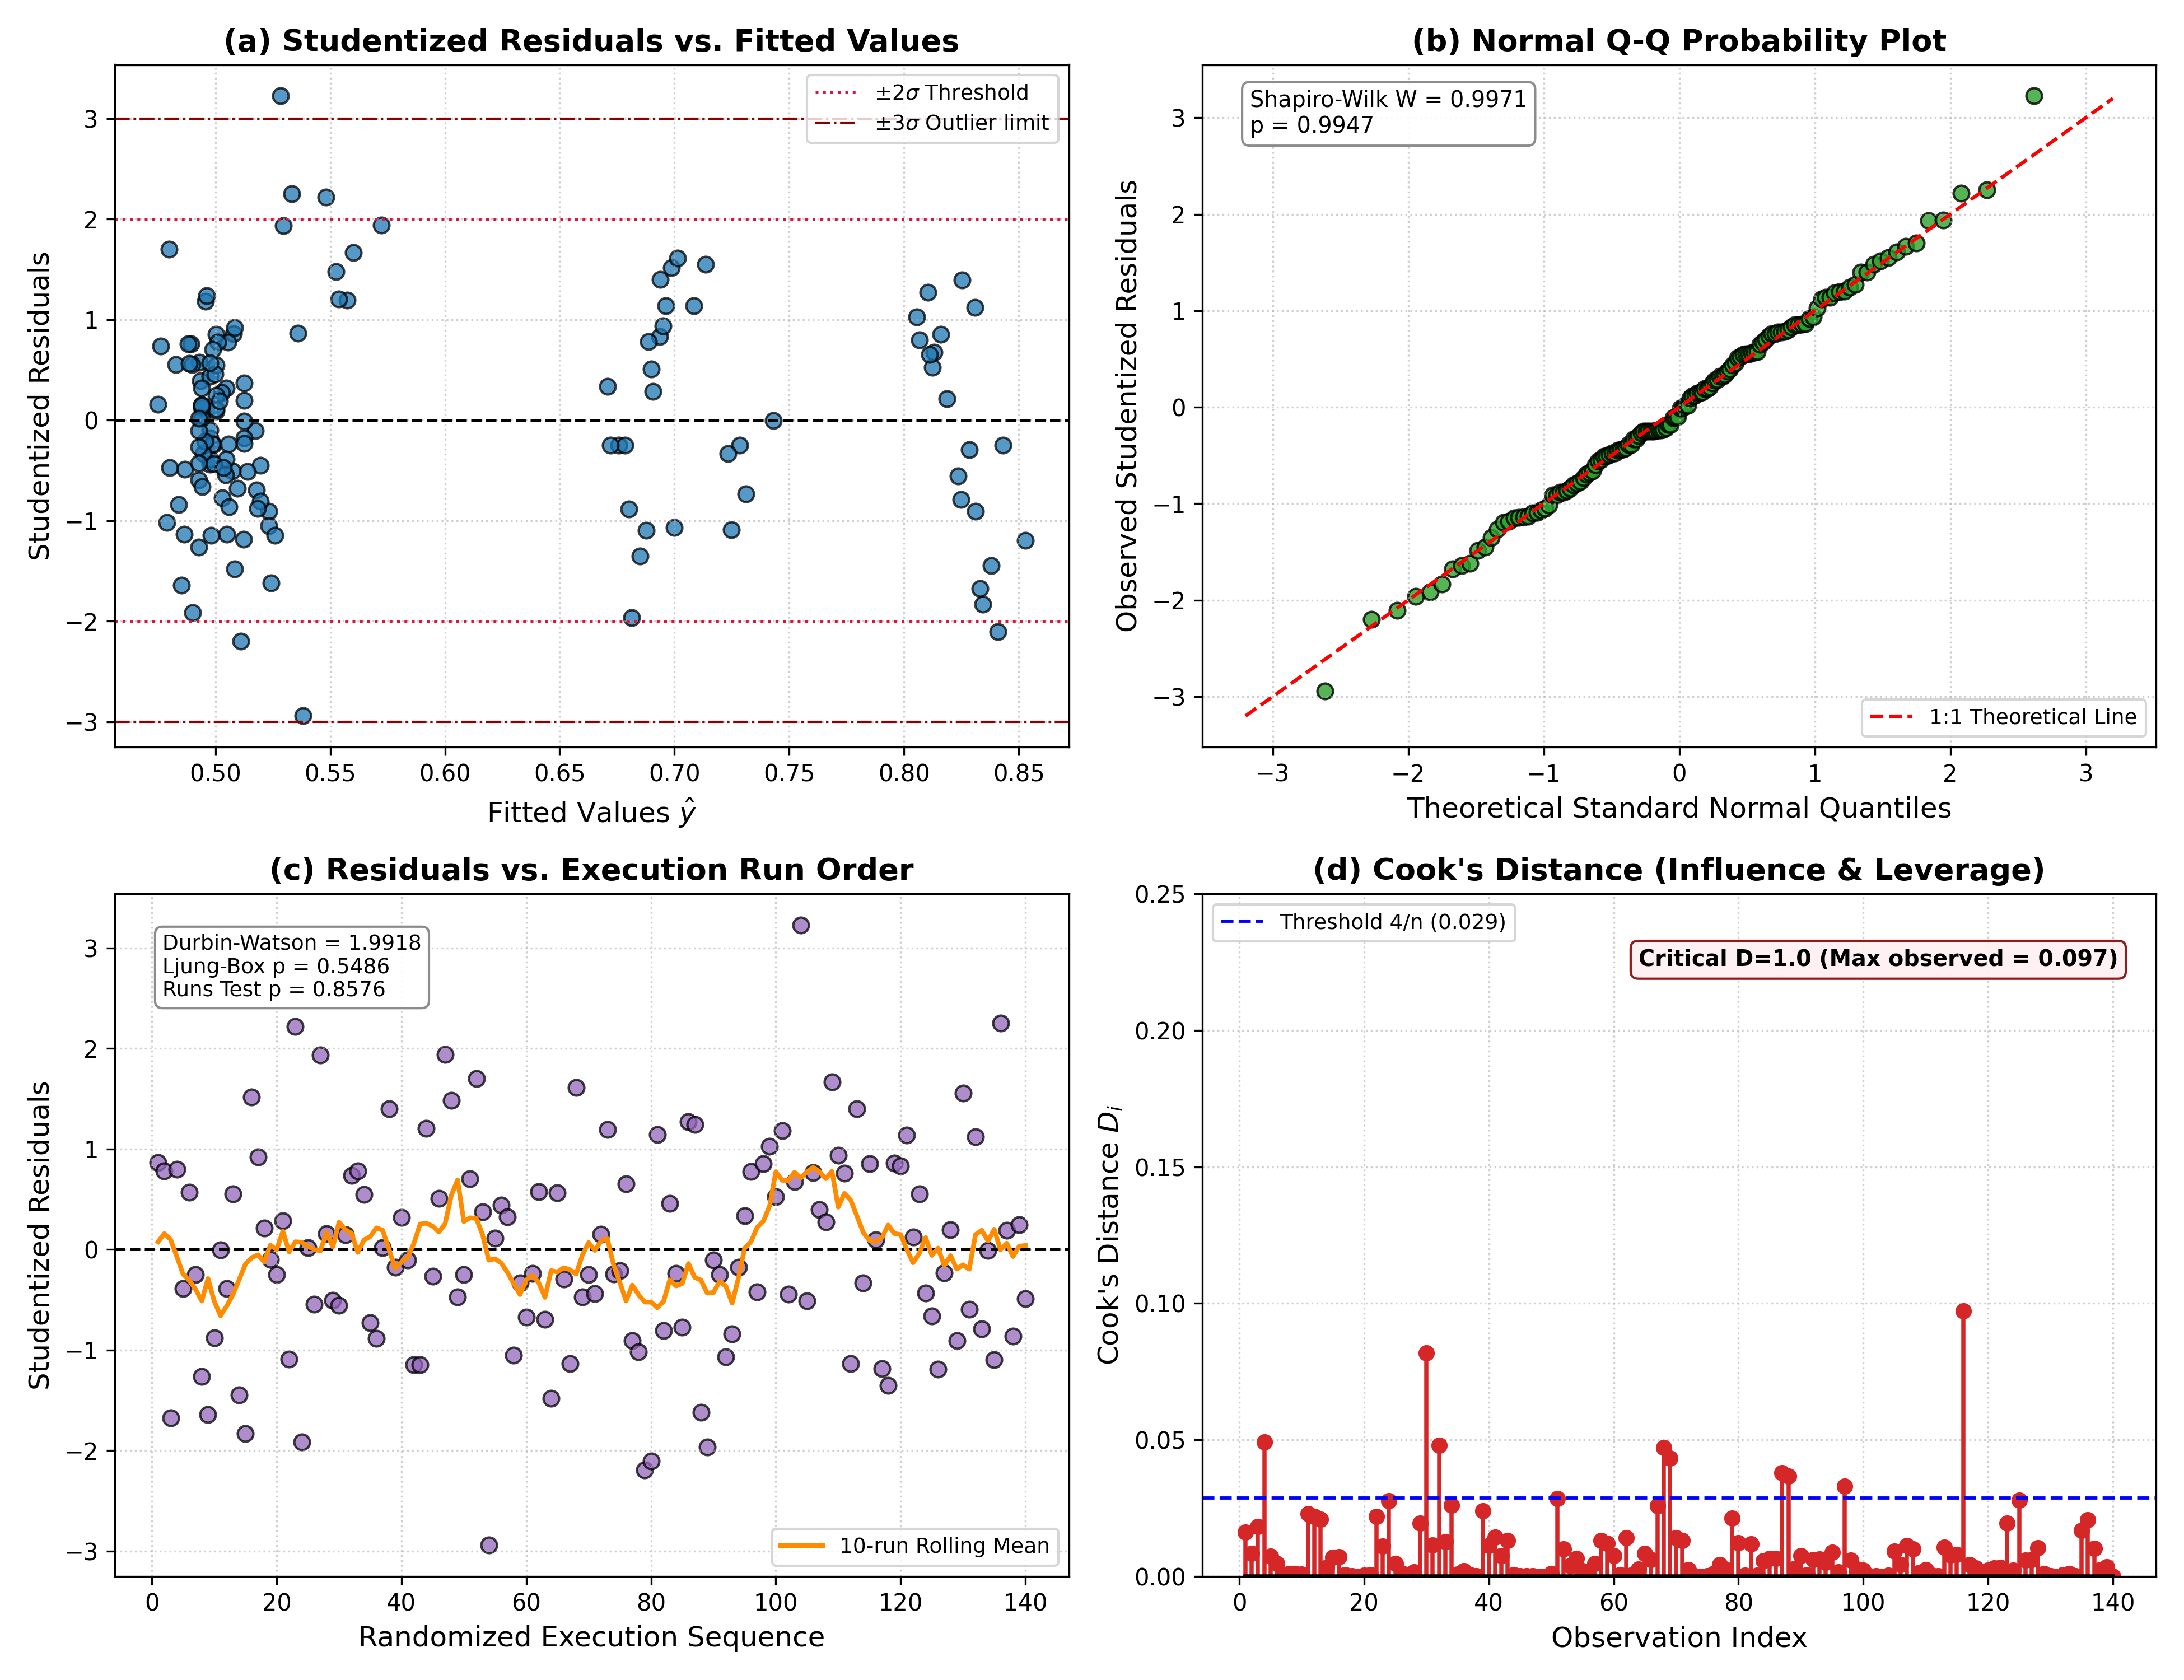
\includegraphics[width=0.95\textwidth]{figures/diagnostics_panel_4in1.png}
\caption{Residual Diagnostics Panel for Second-Order Validation RMSE Model: (a) Studentized residuals vs. fitted values; (b) Normal Q-Q probability plot ($p = \numShapiroP$); (c) Residuals vs. randomized run execution order ($DW = \numDurbinWatson$, Ljung-Box $p = \numLjungBoxP$, Runs test $p = \numRunsTestP$); (d) Cook's distance influence plot bounded well within $D = 1.0$ ($D_{\max} = \numMaxCooksD$).}
\label{fig:diagnostics_panel}
\end{figure}

\section{Phase 3: Canonical and Ridge Analysis}

\subsection{Matrix Representation and Stationary Point}

The fitted second-order model is expressed in matrix notation:
\begin{equation}
    \hat{y} = b_0 + \mathbf{x}^T \mathbf{b} + \mathbf{x}^T \mathbf{B} \mathbf{x}
\end{equation}
where $b_0 = \numBzero$ (averaging block effects equally), $\mathbf{b} = [\vecBOne, \vecBTwo, \vecBThree, \vecBFour]^T$, and:
\begin{equation}
    \mathbf{B} = \begin{bmatrix}
        \matBOneOne & \matBOneTwo & \matBOneThree & \matBOneFour \\
        \matBTwoOne & \matBTwoTwo & \matBTwoThree & \matBTwoFour \\
        \matBThreeOne & \matBThreeTwo & \matBThreeThree & \matBThreeFour \\
        \matBFourOne & \matBFourTwo & \matBFourThree & \matBFourFour
    \end{bmatrix}
\end{equation}
The unconstrained stationary point $\mathbf{x}_0$ satisfies $\mathbf{b} + 2\mathbf{B}\mathbf{x}_0 = \mathbf{0}$:
\begin{equation}
    \mathbf{x}_0 = -\frac{1}{2} \mathbf{B}^{-1} \mathbf{b} = [\numStationaryXone, \numStationaryXtwo, \numStationaryXthree, \numStationaryXfour]^T
\end{equation}
The stationary coordinate along $x_3$ ($\numStationaryXthree$) lies far outside the operational cube $[-1, +1]^4$, with a Euclidean coded distance of $\|\mathbf{x}_0\| = \numStationaryDistCoded$. The unconstrained predicted value $\hat{y}_0 = \numStationaryYhat$ represents an extrapolation artifact.

\subsection{Spectral Decomposition and Ridge Analysis}

Eigenvalues of $\mathbf{B}$ are $\lambda_1 = \numEigOne, \lambda_2 = \numEigTwo, \lambda_3 = \numEigThree, \lambda_4 = \numEigFour$ ($\sum \lambda_i = \text{trace}(\mathbf{B}) = \numTraceB$). While point estimates are positive, Rademacher wild bootstrap (2,000 replications) reveals that the 95\% bootstrap interval for $\lambda_1$ spans $[\numBootLowEigOne, \numBootHighEigOne]$, with $\numFracMinEigLeZero$ of bootstrap samples yielding $\min(\lambda) \le 0$. The system is classified as a \textbf{stationary or rising ridge}, with curvature along $x_3$ and $x_4$ indistinguishable from zero.

Constrained optimization over the hypercube $[-1, 1]^4$ with integer depth $d \in \{3, \dots, 9\}$ yields the results in Table \ref{tab:depth_opt}.

\begin{table}[H]
\centering
\renewcommand{\arraystretch}{1.25}
\setlength{\tabcolsep}{6pt}
\begin{tabular}{cccccccc}
\toprule
\textbf{Depth} & \makecell{\textbf{Coded}\\\bm{$x_1$}} & \makecell{\textbf{Coded}\\\bm{$x_2$}} & \makecell{\textbf{Coded}\\\bm{$x_3$}} & \makecell{\textbf{Coded}\\\bm{$x_4$}} & \makecell{\textbf{Optimal}\\\bm{$\eta$}} & \makecell{\textbf{Predicted}\\\textbf{RMSE}} & \makecell{\textbf{SE}\\\bm{$(\hat{y})$}} \\
\midrule
3 & $0.8103$ & $-1.0000$ & $1.00$ & $1.00$ & $0.2173$ & $0.4909$ & $0.0032$ \\
4 & $0.7573$ & $-0.6667$ & $1.00$ & $1.00$ & $0.1985$ & $0.4724$ & $0.0030$ \\
5 & $0.7043$ & $-0.3333$ & $1.00$ & $1.00$ & $0.1814$ & $0.4592$ & $0.0032$ \\
6 & $0.6513$ & $+0.0000$ & $1.00$ & $1.00$ & $0.1658$ & $0.4511$ & $0.0033$ \\
7 & $0.5983$ & $+0.3333$ & $1.00$ & $1.00$ & $0.1515$ & $0.4483$ & $0.0032$ \\
8 & $0.5453$ & $+0.6667$ & $1.00$ & $1.00$ & $0.1384$ & $0.4506$ & $0.0031$ \\
9 & $0.4923$ & $+1.0000$ & $1.00$ & $1.00$ & $0.1265$ & $0.4582$ & $0.0034$ \\
\bottomrule
\end{tabular}

\vspace{0.6em}
\caption{Best Predicted Validation RMSE at Each Discrete Tree Depth}
\label{tab:depth_opt}
\end{table}

The constrained single-objective optimum within the hypercube occurs at depth $\numCubeOptDepth$ ($x_1 = \numCubeOptXone, x_2 = \numCubeOptXtwo, x_3 = \numCubeOptXthree, x_4 = \numCubeOptXfour$) with predicted RMSE $\numCubeOptPredRMSE$. Figures \ref{fig:surface_rmse} and \ref{fig:latency_depth} display the response surfaces.

\begin{figure}[H]
\centering
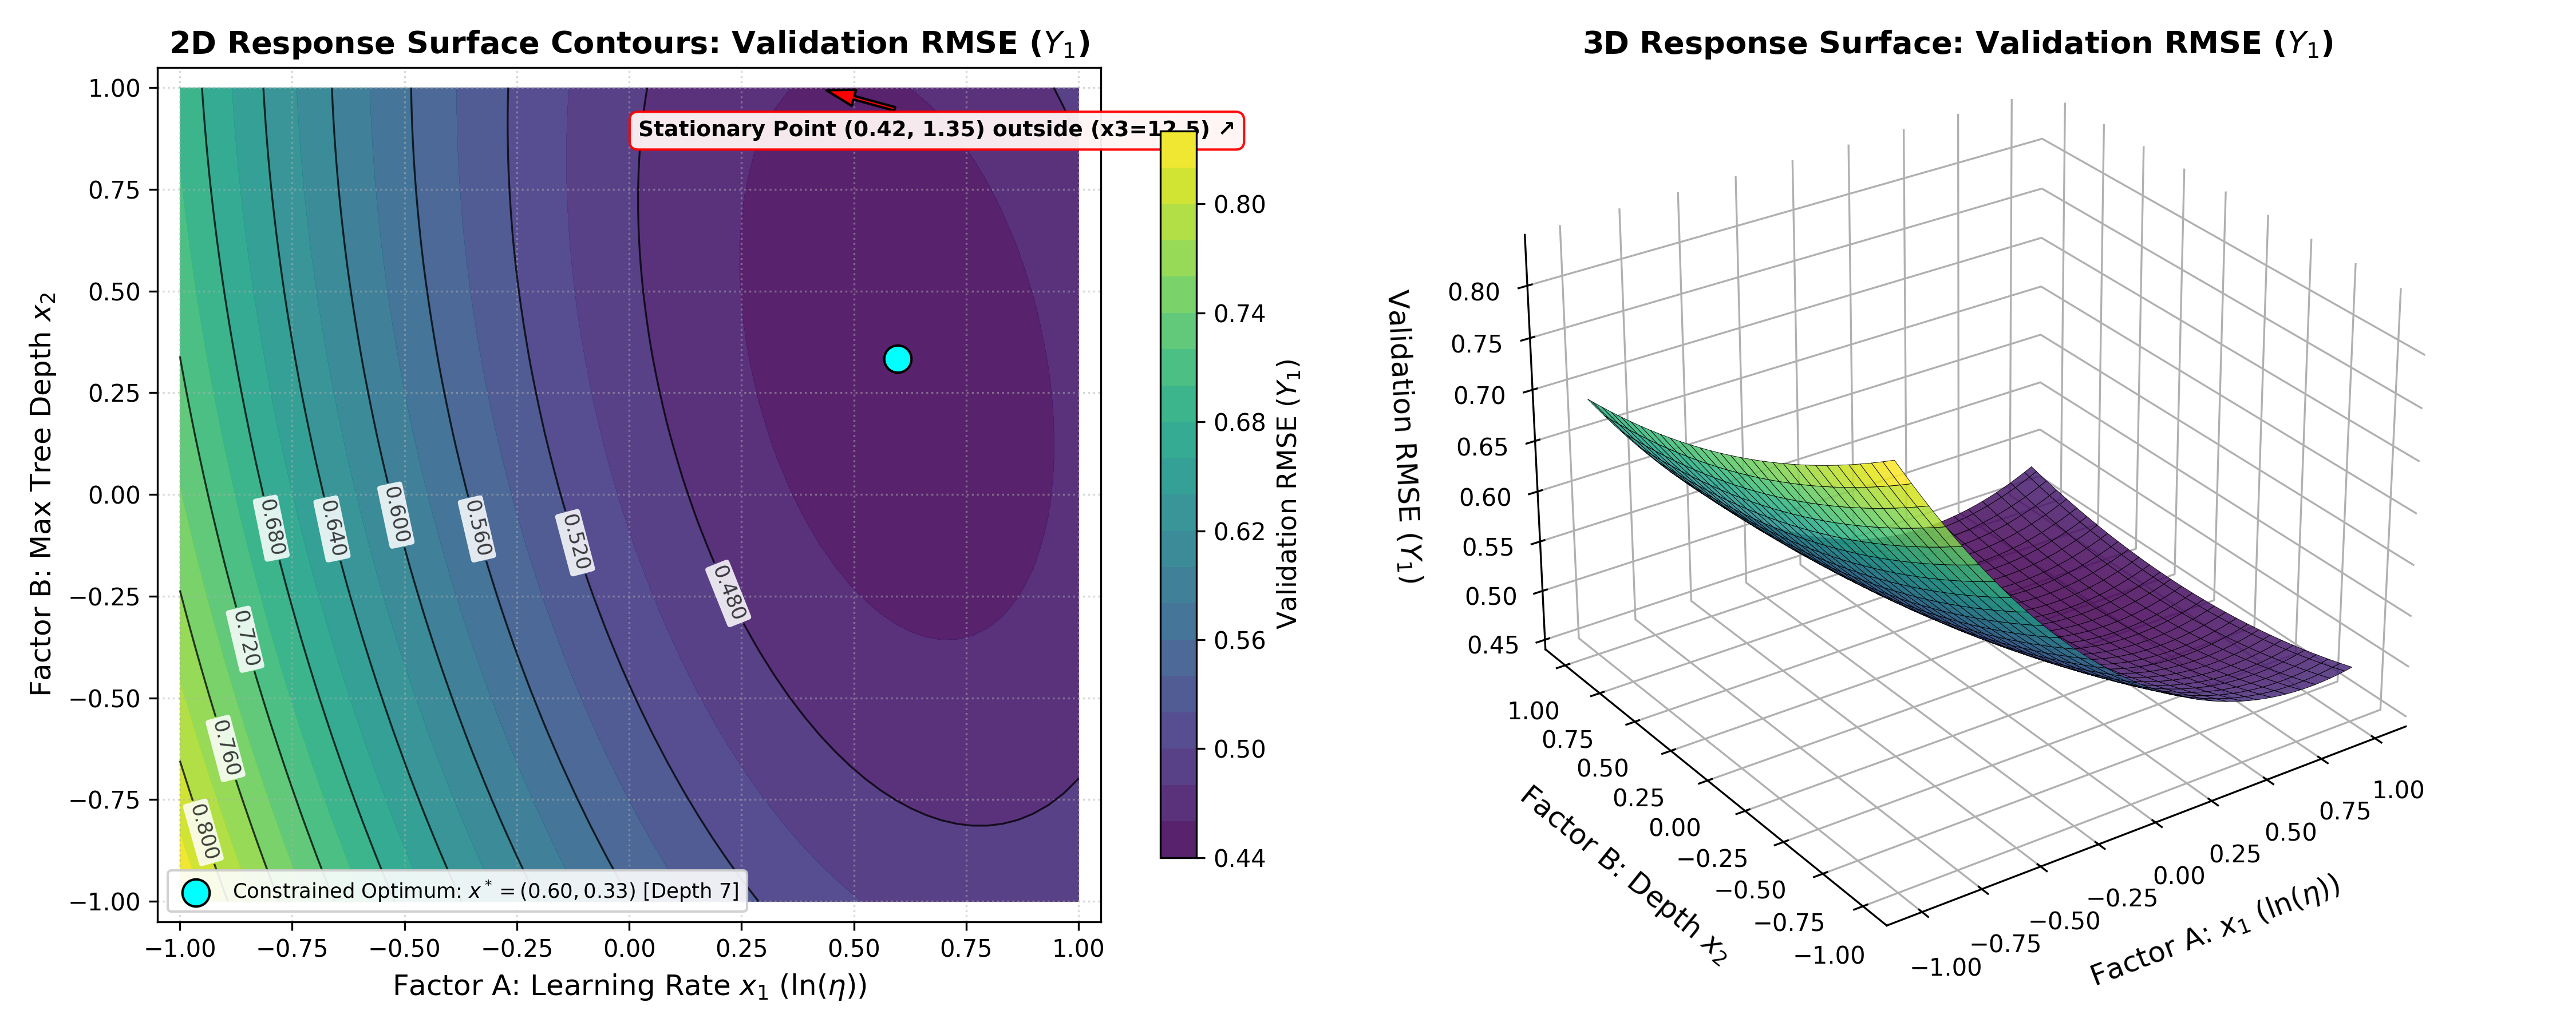
\includegraphics[width=0.95\textwidth]{figures/response_surface_rmse_2d_3d.png}
\caption{Response Surface Topography for Validation RMSE ($Y_1$): (a) 2D contour slice across Factor A ($\ln(\eta)$) and Factor B (depth), passing through the constrained optimum ($x_3=1, x_4=1$). Arrow indicates trajectory toward unconstrained stationary point outside domain; (b) 3D wireframe projection.}
\label{fig:surface_rmse}
\end{figure}

\begin{figure}[H]
\centering
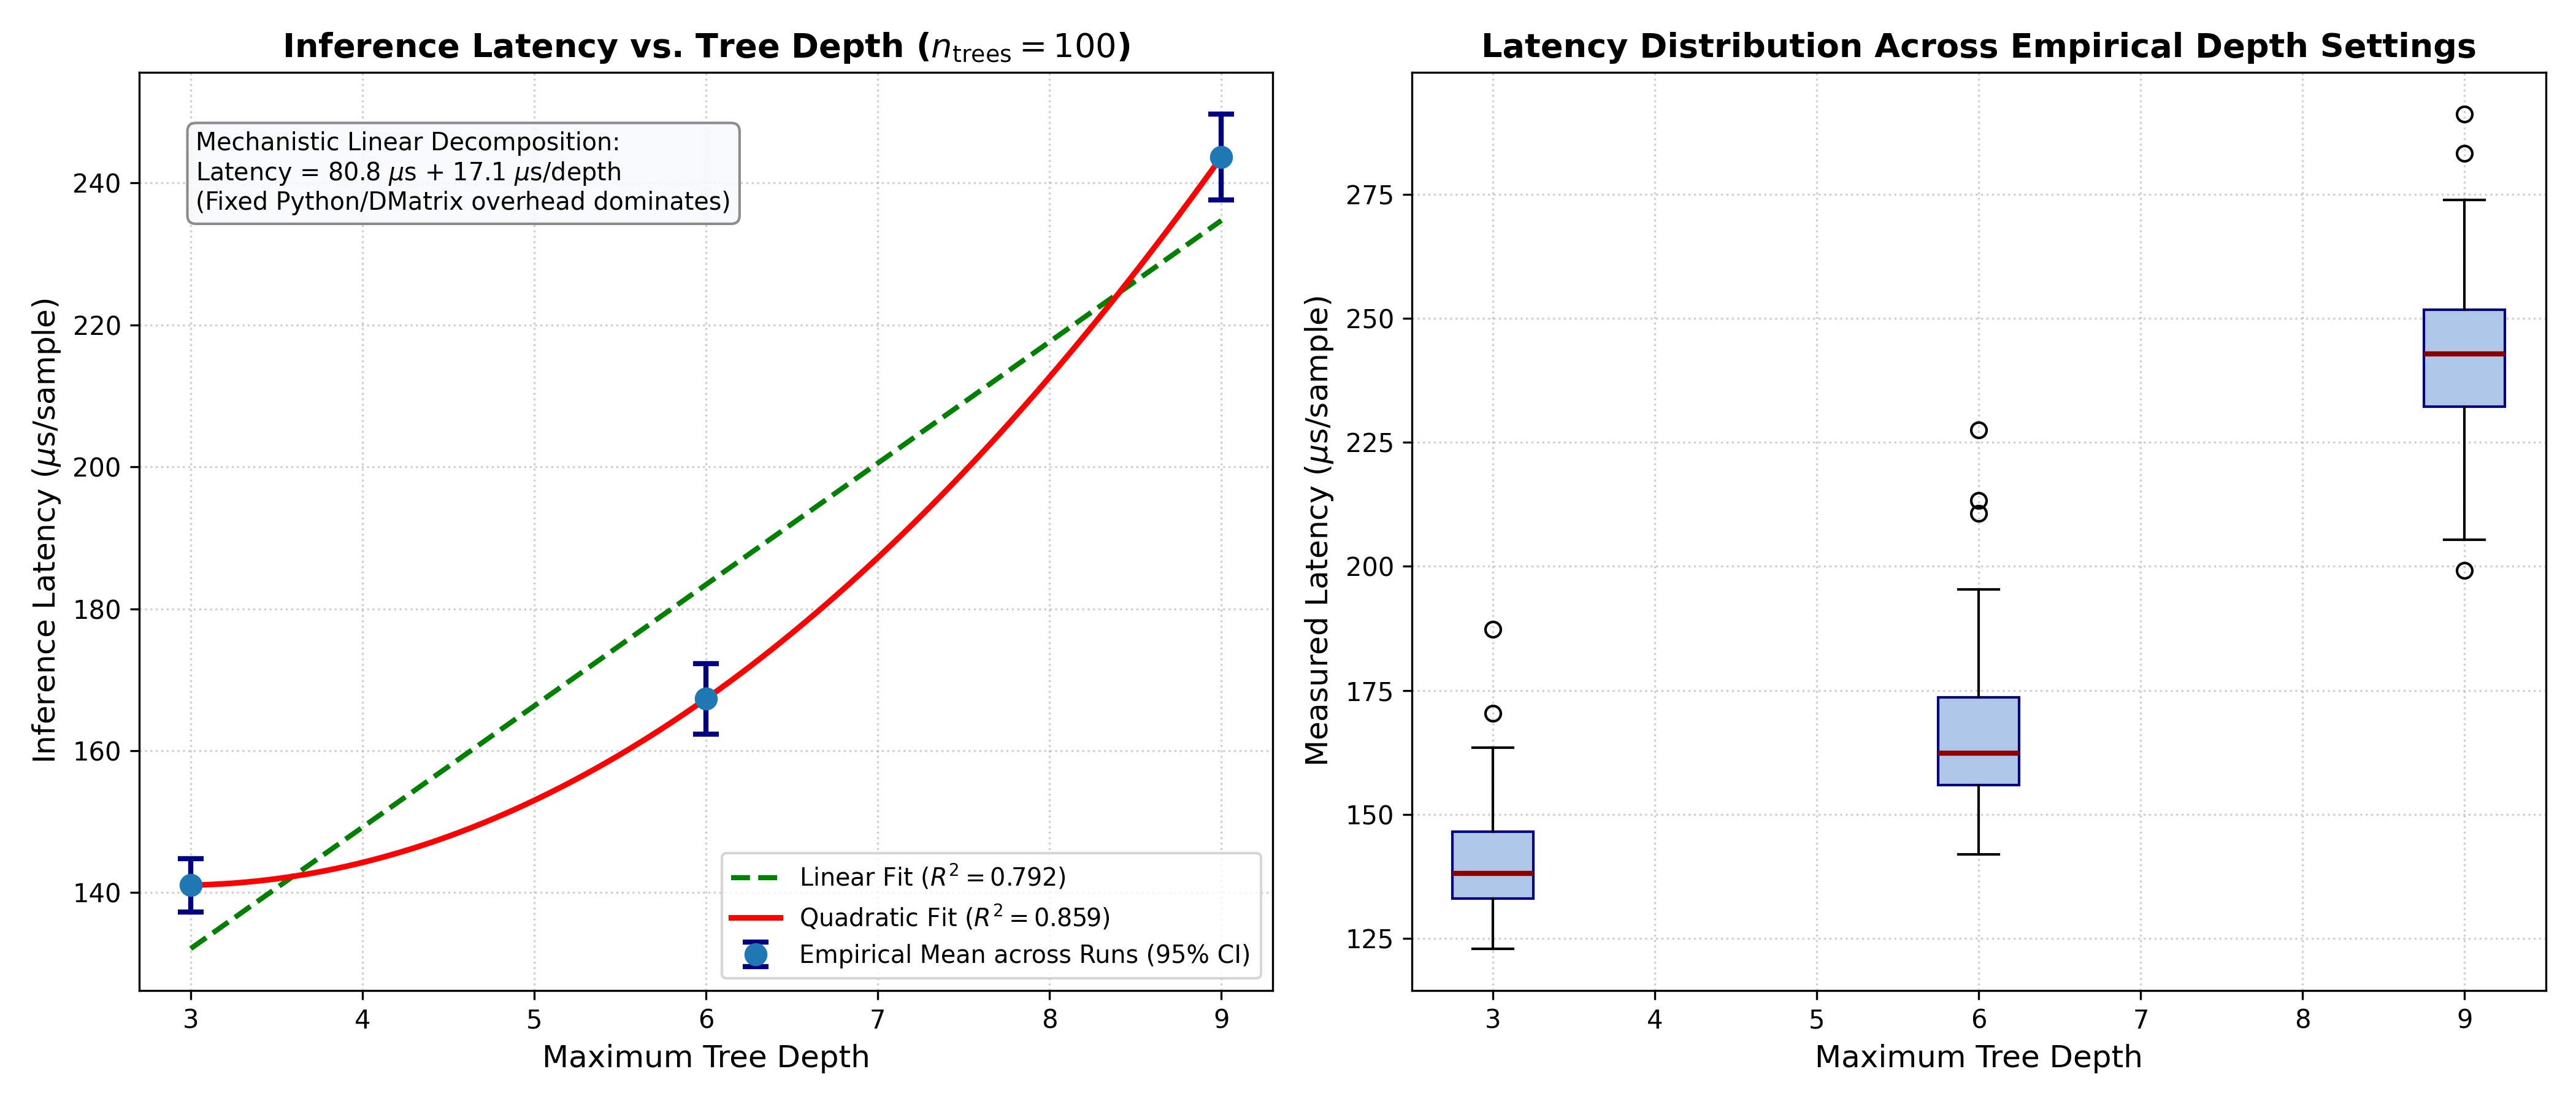
\includegraphics[width=0.95\textwidth]{figures/response_surface_latency_2d_3d.png}
\caption{Inference Latency Modelling: (a) Empirical mean latency with 95\% CI error bars vs. linear ($R^2 = \numLatLinRsq$) and quadratic ($R^2 = \numLatQuadRsq$) fits. Note the substantial fixed overhead ($\approx 105\ \mu\text{s}$) arising from Python execution and tree traversal; (b) Distribution boxplots across discrete depths.}
\label{fig:latency_depth}
\end{figure}

\section{Phase 4: Multi-Objective Desirability Optimization}

Minimizing predictive error requires deeper trees, which increases inference latency. To identify a principled compromise, we employ Derringer-Suich desirability functions \cite{derringer1980simultaneous}:
\begin{equation}
    d_r(Y_r) = \begin{cases}
        1.0, & Y_r < L_r \\
        \left(\frac{U_r - Y_r}{U_r - L_r}\right)^{s_r}, & L_r \le Y_r \le U_r \\
        0.0, & Y_r > U_r
    \end{cases}
\end{equation}
The composite desirability $D$ is formulated with explicit importance weights $(w_1, w_2)$:
\begin{equation}
    D = \left( d_1(Y_1)^{w_1} \cdot d_2(Y_2)^{w_2} \right)^{\frac{1}{w_1 + w_2}}
\end{equation}
In the baseline scenario, equal weights $w_1 = 1, w_2 = 1$ are utilized with engineering limits $L_1 = 0.450, U_1 = 0.700$ for RMSE and $L_2 = 100.0, U_2 = 180.0\ \mu\text{s}$ for latency ($s_1 = s_2 = 1.0$). Maximizing $D$ over $[-1, 1]^4$ with integer depth yields the optimum:
\begin{align}
    \mathbf{x}^* &= [\numOptXone, \numOptXtwo, \numOptXthree, \numOptXfour]^T \nonumber \\
    &\implies (\eta = \numOptEta, \text{depth} = \numOptDepth, \text{subsample} = \numOptSubsample, \lambda = \numOptLambda)
\end{align}
achieving $D = \numOptD$ ($d_1 = \numOptdOne, d_2 = \numOptdTwo$). Predicted metrics at $\mathbf{x}^*$ are $\hat{Y}_1 = \numPredRMSE$ and $\hat{Y}_2 = \numPredLatency\ \mu\text{s}$. Table \ref{tab:desirability_sensitivity} presents sensitivity analysis across alternative specification limits and weightings.

\begin{table}[H]
\centering
\renewcommand{\arraystretch}{1.25}
\setlength{\tabcolsep}{4pt}
\begin{tabular}{lcccccc}
\toprule
\textbf{Scenario} & \makecell{\textbf{RMSE Bounds}\\\bm{$[L_1, U_1]$}} & \makecell{\textbf{Latency Bounds}\\\bm{$[L_2, U_2]$}} & \makecell{\textbf{Weights}\\\bm{$(w_1, w_2)$}} & \makecell{\textbf{Opt}\\\textbf{Depth}} & \makecell{\textbf{Opt}\\\bm{$\eta$}} & \makecell{\textbf{Best}\\\bm{$D$}} \\
\midrule
Standard Config & [0.45, 0.70] & [100, 180] & (1, 1) & 4 & $0.3000$ & $0.6952$ \\
Strict Latency & [0.45, 0.70] & [90, 140] & (1, 2) & 3 & $0.3000$ & $0.2206$ \\
Strict Accuracy & [0.44, 0.60] & [100, 200] & (2, 1) & 5 & $0.2135$ & $0.7293$ \\
Narrow Range & [0.46, 0.65] & [110, 160] & (1, 1) & 4 & $0.3000$ & $0.6597$ \\
\bottomrule
\end{tabular}

\vspace{0.6em}
\caption{Desirability Optimization Sensitivity Analysis Across Bounds and Weights}
\label{tab:desirability_sensitivity}
\end{table}

Figure \ref{fig:pareto_front} illustrates the empirical Pareto frontier and the location of $\mathbf{x}^*$.

\begin{figure}[H]
\centering
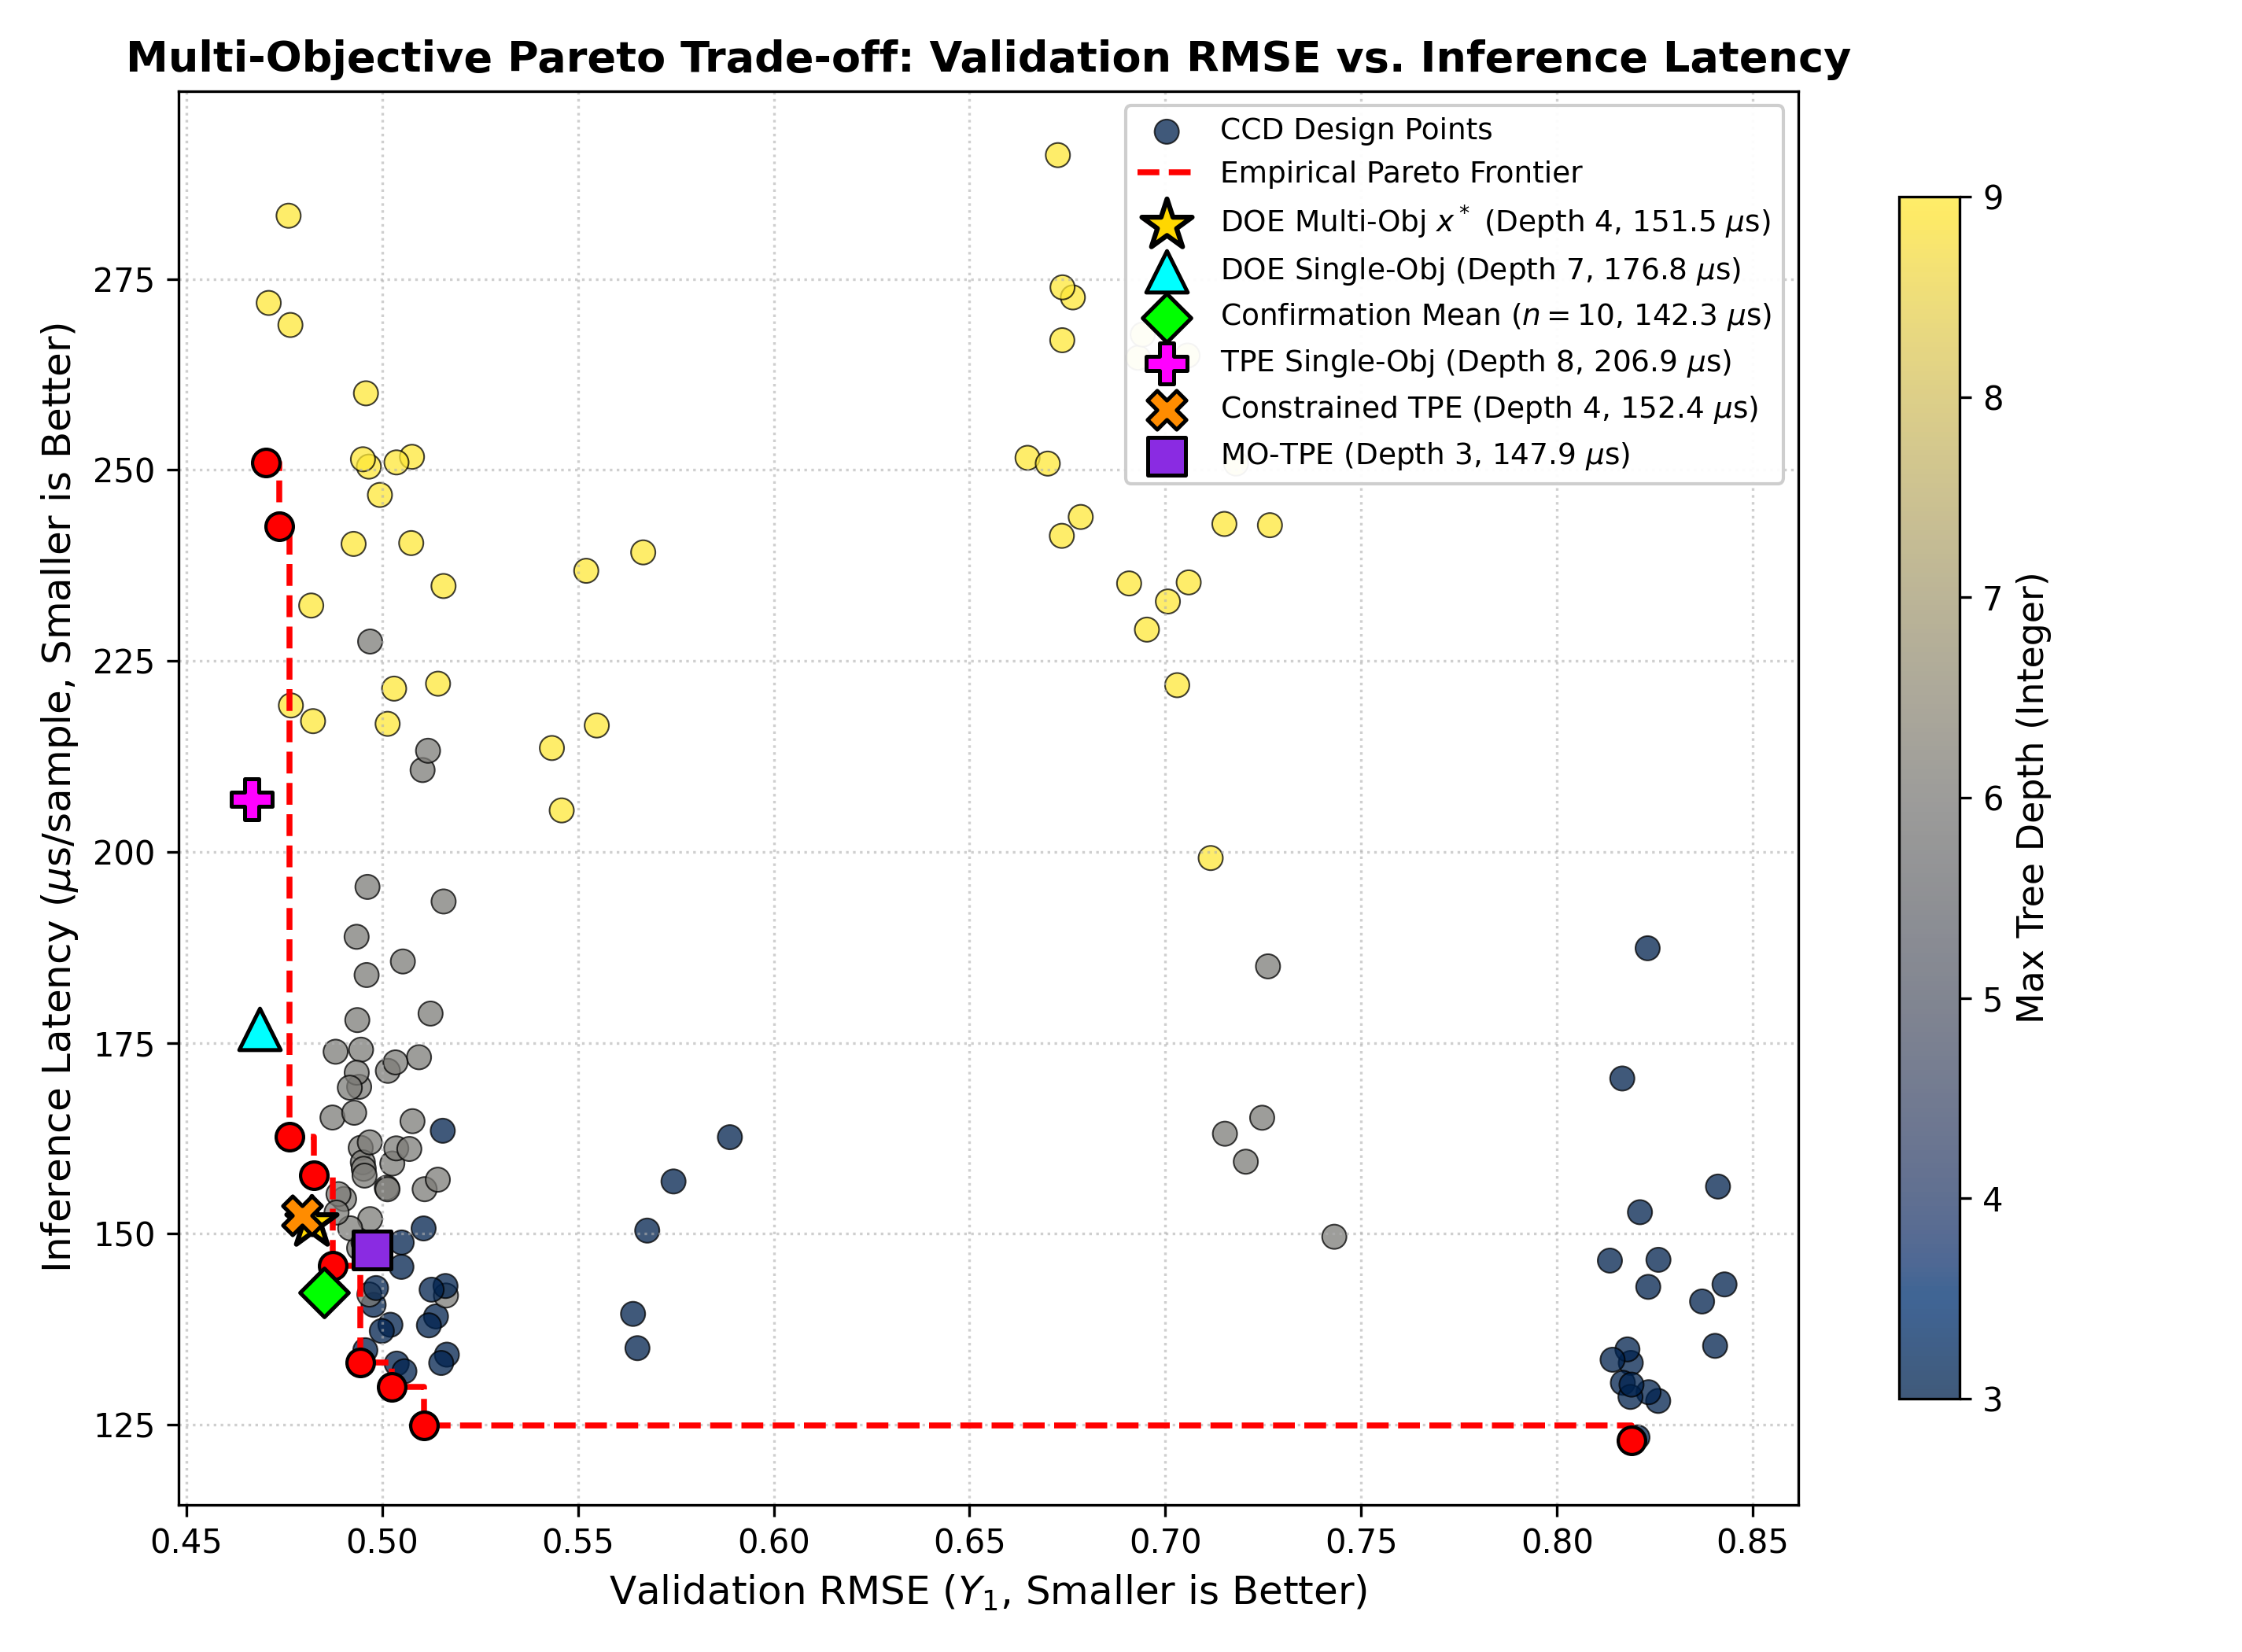
\includegraphics[width=0.80\textwidth]{figures/desirability_pareto_front.png}
\caption{Multi-Objective Pareto Trade-off between Validation RMSE and Inference Latency. Scatter points from CCD design are colored by tree depth using cividis. The empirical Pareto frontier is traced in red, with DOE multi-objective optimum $\mathbf{x}^*$ (depth 4), DOE single-objective optimum (depth 7), confirmation means ($n=10$), and benchmark incumbents highlighted.}
\label{fig:pareto_front}
\end{figure}

\section{Phase 5: Empirical Confirmation and Benchmark Comparison}

\subsection{Confirmation Experiments at Multi-Objective and Single-Objective Optima}

To test surrogate fidelity, $m = 10$ confirmation trials were executed at $\mathbf{x}^*$ across fresh seeds disjoint from the design ($\mathcal{S}_{\text{conf}} = \{505, \dots, 1414\}$). To account for the fact that fresh seeds carry block variance, the 95\% prediction interval incorporates both parameter covariance and block variance:
\begin{equation}
    \text{PI}_{0.95}(\hat{y}) = \hat{y} \pm t_{0.025, 121} \sqrt{\text{MS}_E \left(1 + \mathbf{x}^T (\mathbf{X}^T \mathbf{X})^{-1} \mathbf{x}\right) + \sigma^2_{\text{block}}\left(\frac{1}{m} + \frac{1}{5}\right)}
\end{equation}
In addition, we confirmed the single-objective optimum (depth 7) to directly evaluate model bias against empirical performance. Table \ref{tab:confirmation} compares predictions against empirical results.

\begin{table}[H]
\centering
\renewcommand{\arraystretch}{1.25}
\setlength{\tabcolsep}{3.5pt}
\begin{tabular}{lcccc}
\toprule
\makecell[l]{\textbf{Configuration /}\\\textbf{Response Metric}} & \makecell{\textbf{Surrogate}\\\textbf{Pred ($\hat{y}$)}} & \makecell{\textbf{95\% Pred}\\\textbf{Interval (PI)}} & \makecell{\textbf{Empirical}\\\textbf{Mean $\pm$ SD}} & \makecell{\textbf{Confirmation}\\\textbf{Status}} \\
\midrule
\multicolumn{5}{l}{\textbf{DOE Multi-Objective Optimum $x^*$ (Depth 4)}} \\
Validation RMSE ($Y_1$) & $0.4804$ & $[0.4687, 0.4922]$ & $0.4853 \pm 0.0115$ & \makecell[c]{\textbf{Pass}\\(Inside 95\% PI)} \\
Holdout Test RMSE & --- & --- & $0.4888 \pm 0.0032$ & Holdout Test Set \\
Inference Latency ($\mu$s) & $138.1$ & $[122.8, 153.4]$ & $142.3 \pm 7.8$ & \makecell[c]{\textbf{Pass}\\(Inside 95\% PI)} \\
\midrule
\multicolumn{5}{l}{\textbf{DOE Single-Objective Optimum (Depth 7)}} \\
Validation RMSE ($Y_1$) & $0.4483$ & $[0.4363, 0.4603]$ & $0.4700 \pm 0.0093$ & \makecell[c]{\textbf{Empirical Opt}\\(Bias: +0.0217)} \\
Holdout Test RMSE & --- & --- & $0.4691 \pm 0.0034$ & Holdout Test Set \\
Inference Latency ($\mu$s) & $187.0$ & $[171.1, 202.9]$ & $171.1 \pm 10.9$ & Verified Scale \\
\bottomrule
\end{tabular}

\vspace{0.6em}
\caption{Model Prediction vs. Empirical Confirmation Trials ($m=10$ Fresh Seeds)}
\label{tab:confirmation}
\end{table}

For the multi-objective optimum $\mathbf{x}^*$ (depth 4), the empirical validation RMSE of $\numConfEmpValRMSE \pm \numConfEmpValRMSEStd$ falls directly inside the 95\% prediction interval ($[\numConfPiLowValRMSE, \numConfPiHighValRMSE]$), confirming surrogate validity. Empirical latency was $\numConfEmpLat \pm \numConfEmpLatStd\ \mu\text{s}$, also falling well within $[122.8, 153.4]\,\mu\text{s}$. Generalization test RMSE evaluated on the untouched external holdout set ($N=4,128$) averaged $\numConfEmpTestRMSE \pm \numConfEmpTestRMSEStd$.

For the single-objective optimum (depth 7), empirical validation RMSE was $\numConfSoEmpValRMSE \pm \numConfSoEmpValRMSEStd$ against a prediction of $\numConfSoPredValRMSE$. The resulting empirical bias of $\numConfSoBias$ is bounded well within the second-order lack-of-fit RMS misfit of $\numSqrtMSLofYone$, proving that the surrogate accurately locates the empirical optimum despite minor interpolation bias at intermediate depth levels.

\subsection{Benchmark Evaluation Against Random Search and Optuna TPE}

We evaluated four baseline configurations against the DOE recommended optima under equal-budget conditions (140 function evaluations):
\begin{enumerate}
    \item \textbf{Unguided Random Search:} 20 independent runs of 140 evaluations.
    \item \textbf{Single-Objective TPE:} 20 independent runs of 140 evaluations optimizing validation RMSE.
    \item \textbf{Constrained TPE:} Single-objective TPE with latency constraint ($\le 145\,\mu\text{s}$) strictly enforced during search.
    \item \textbf{Multi-Objective TPE:} Optimizes validation RMSE and latency simultaneously.
\end{enumerate}

Final incumbents from each method were evaluated across 20 fresh seeds (seeds $2001$--$2020$, $\mathcal{S}_{\text{eval}}$) on the fixed holdout test set with pinned CPU core affinity and interleaved repeats. Table \ref{tab:benchmarks} summarizes the benchmark comparison.

\begin{table}[H]
\centering
\renewcommand{\arraystretch}{1.25}
\setlength{\tabcolsep}{2pt}
\begin{tabular}{lcccccc}
\toprule
\makecell{\textbf{Optimization Method}} & \makecell{\textbf{Search Basis}\\\scriptsize\textbf{($N$ Replicates)}} & \makecell{\textbf{Val RMSE}\\\scriptsize\textbf{Mean $\pm$ SD$_{\text{search}}$}} & \makecell{\textbf{Holdout Test RMSE}\\\scriptsize\textbf{Mean $\pm$ SD$_{\text{search}}$}} & \makecell{\textbf{Retrain}\\\bm{$\sigma_{\text{eval}}$}} & \makecell{\textbf{Predict Latency}\\\bm{$(\mu\text{s} \pm \text{SD})$}} & \makecell{\textbf{Benchmark}\\\textbf{Feasible}} \\
\midrule
\multicolumn{7}{l}{\textbf{Panel A: Prospective Revision-v2 Full Benchmark ($N=20$ Independent Search Replicates, 140 Fits/Rep)}} \\
\makecell[l]{Repeated DOE Multi-Obj ($\mathbf{x}^*_{\text{MO}}$)} & RSM ($N{=}20$ reps) & $0.4853 \pm 0.0055$ & $0.4900 \pm 0.0073$ & $0.0033$ & $122.3 \pm 2.7$ & 20/20 \\
\makecell[l]{Multi-Objective TPE (Desirability)} & Parzen ($N{=}20$ reps) & $0.4881 \pm 0.0093$ & $0.4926 \pm 0.0108$ & $0.0036$ & $121.5 \pm 3.8$ & 20/20 \\
\makecell[l]{Constrained TPE ($\le 145\,\mu\text{s}$)} & Parzen ($N{=}20$ reps) & $0.4700 \pm 0.0022$ & $0.4704 \pm 0.0032$ & $0.0034$ & $144.3 \pm 7.1$ & 9/20 \\
\makecell[l]{Repeated DOE Single-Obj ($\mathbf{x}^*_{\text{SO}}, d{=}7$)} & RSM ($N{=}20$ reps) & $0.4687 \pm 0.0000$ & $0.4686 \pm 0.0000$ & $0.0030$ & $150.7 \pm 0.7$ & 0/20 \\
\makecell[l]{Single-Objective TPE} & Parzen ($N{=}20$ reps) & $0.4675 \pm 0.0008$ & $0.4669 \pm 0.0012$ & $0.0031$ & $188.9 \pm 12.1$ & 0/20 \\
\makecell[l]{Unguided Random Search} & Uniform ($N{=}20$ reps) & $0.4687 \pm 0.0014$ & $0.4695 \pm 0.0021$ & $0.0030$ & $181.1 \pm 19.0$ & 0/20 \\
\midrule
\multicolumn{7}{l}{\textbf{Panel B: Historical Baseline Snapshot ($v1.0.0$, Single Search Replicate)}} \\
\makecell[l]{Historical DOE Multi-Obj ($\mathbf{x}^*_{\text{MO}}$)} & RSM (Single rep) & $0.4821$ & $0.4884$ & --- & $119.8$ & Yes \\
\makecell[l]{Historical Multi-Obj TPE} & Parzen (Single rep) & $0.4812$ & $0.4870$ & --- & $118.8$ & Yes \\
\makecell[l]{Historical Constrained TPE} & Parzen (Single rep) & $0.4783$ & $0.4823$ & --- & $125.4$ & Yes \\
\makecell[l]{Historical DOE Single-Obj ($d{=}7$)} & RSM (Single rep) & $0.4687$ & $0.4690$ & --- & $147.8$ & No \\
\makecell[l]{Historical Bayesian TPE (SO)} & Parzen (Single rep) & $0.4735$ & $0.4726$ & --- & $193.2$ & No \\
\makecell[l]{Historical Random Search} & Uniform (Single rep) & $0.4696$ & $0.4707$ & --- & $198.1$ & No \\
\bottomrule
\end{tabular}

\vspace{0.6em}
\caption{Empirical Benchmark Comparison across 20 Fresh Seeds on Fixed Holdout Test Set}
\label{tab:benchmarks}
\end{table}

Figure \ref{fig:efficiency_curves} illustrates optimization efficiency across training evaluations.

\begin{figure}[H]
\centering
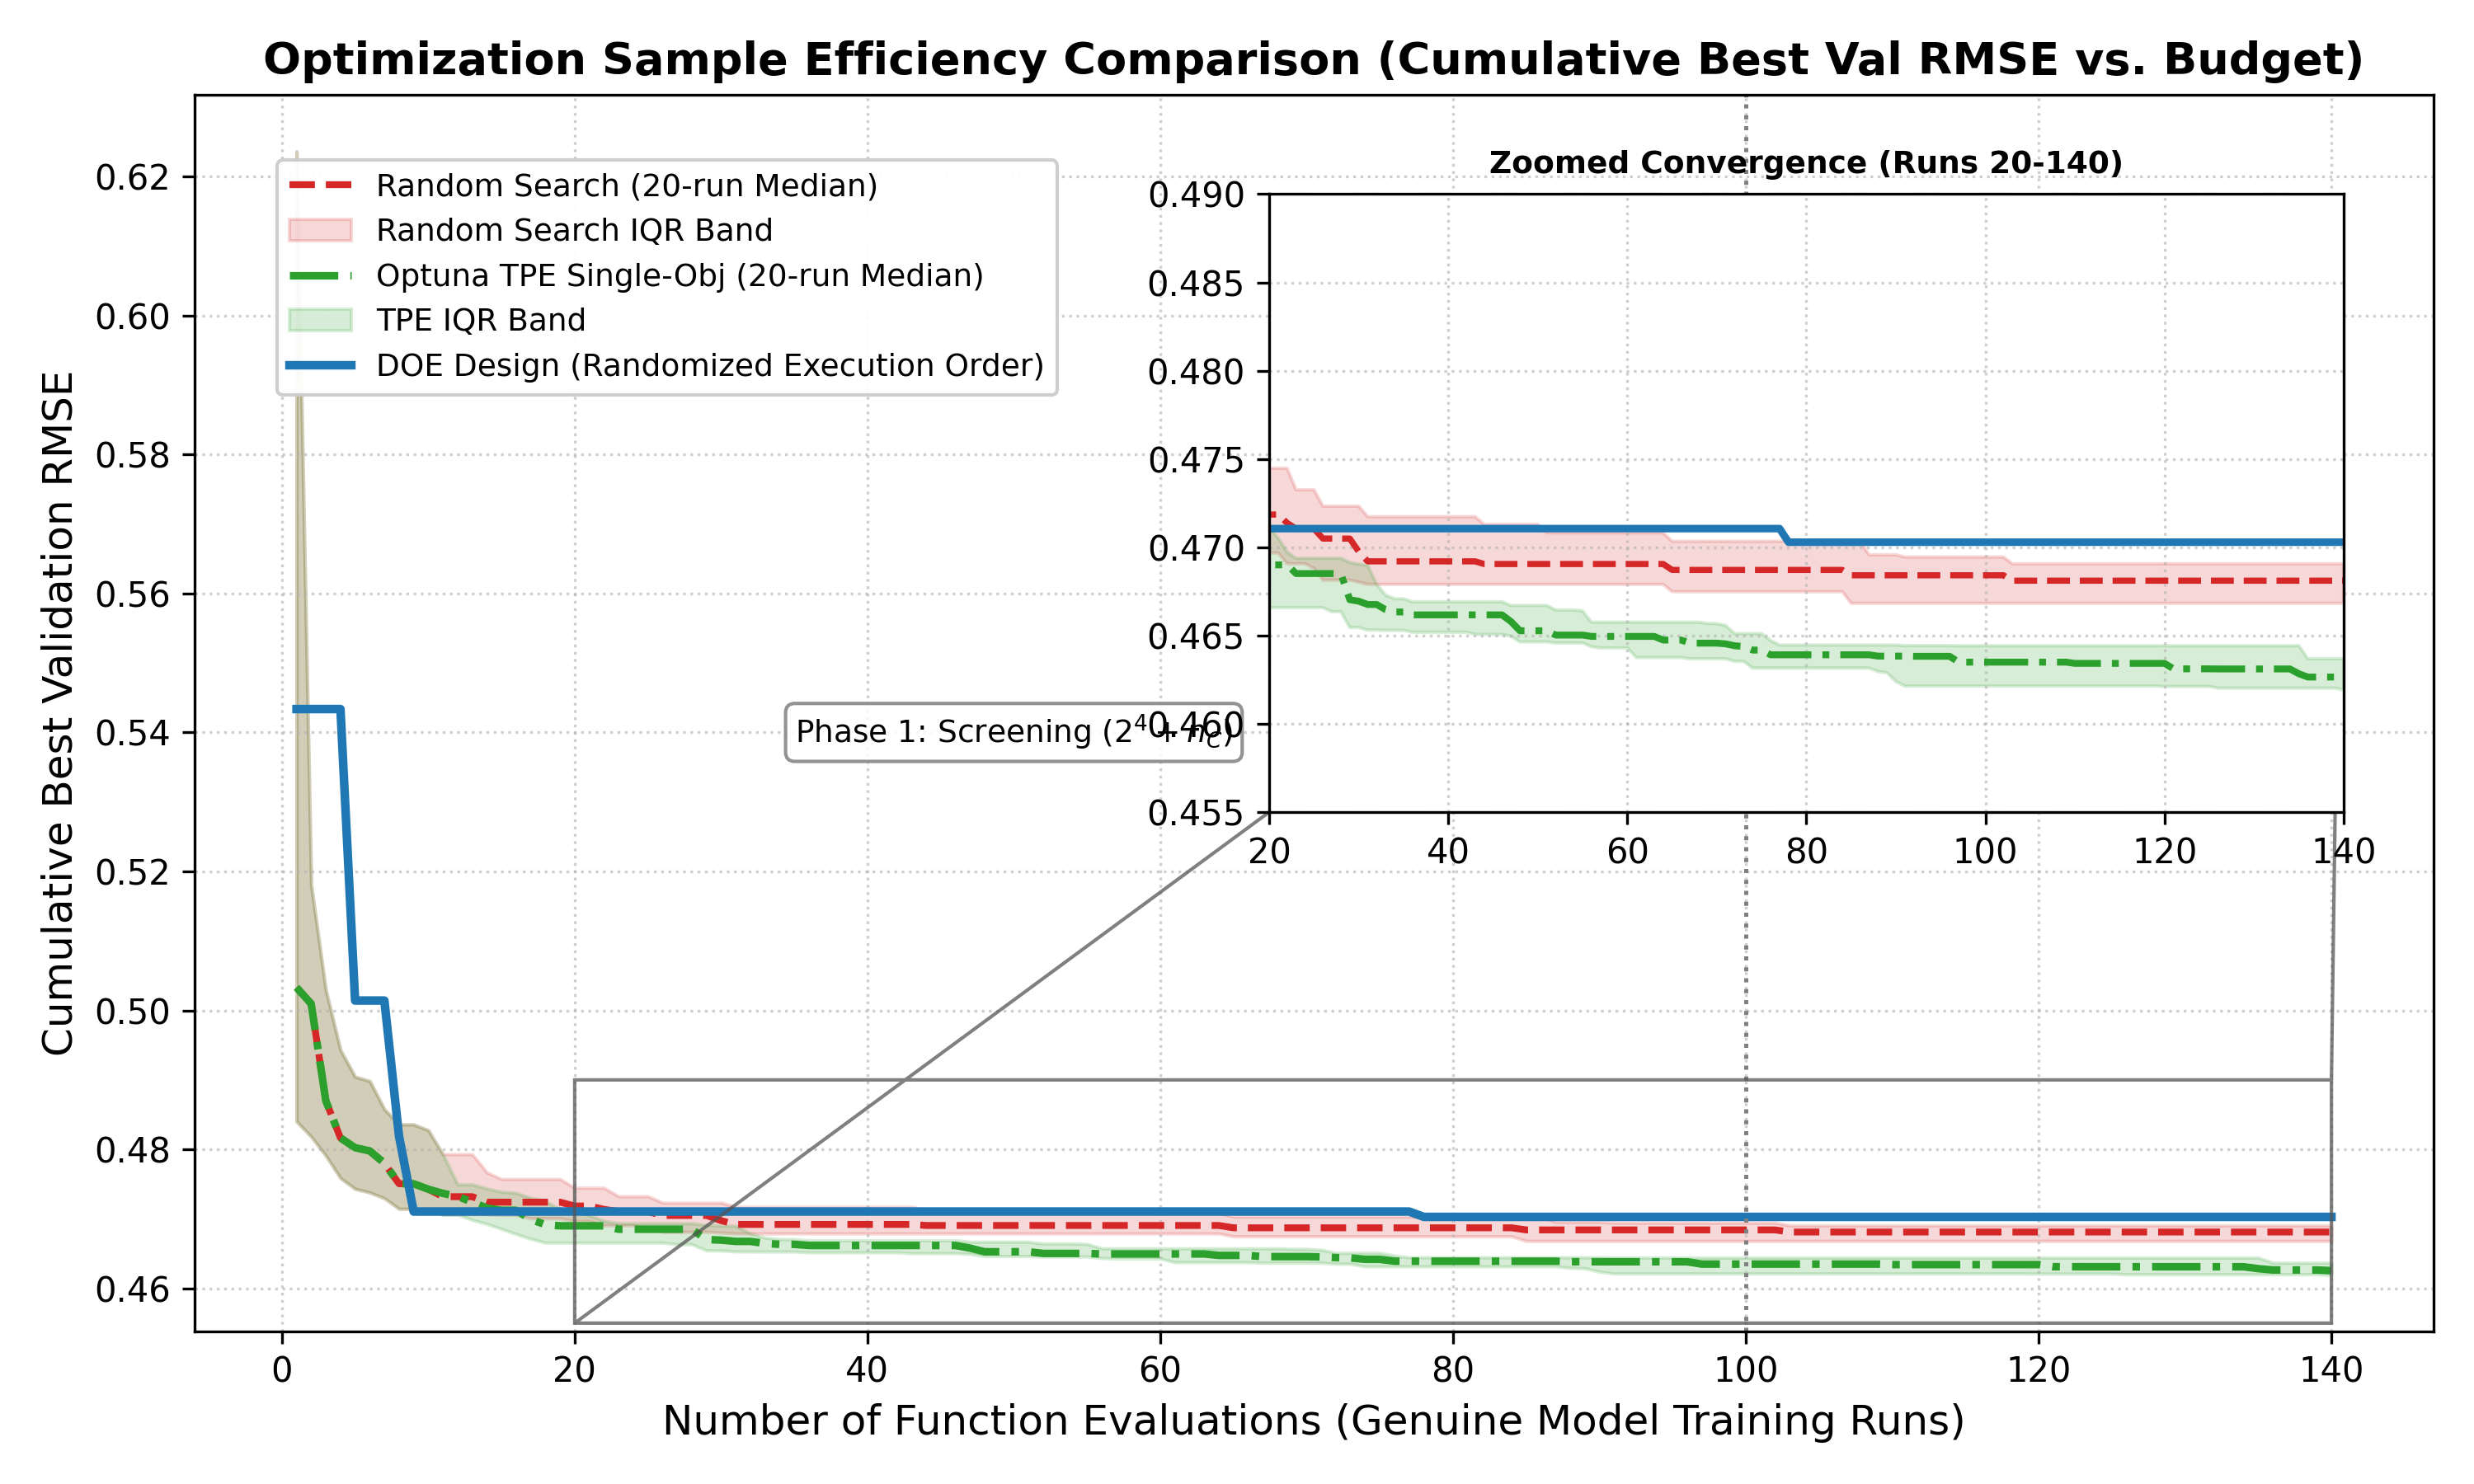
\includegraphics[width=0.92\textwidth]{figures/efficiency_comparison_curve.png}
\caption{Sample Efficiency Convergence: Cumulative best validation RMSE vs. evaluation budget. Curves for Random Search and TPE show median trajectories $\pm$ IQR shaded bands across 20 independent runs. The sequential DOE curve shows cumulative best in actual randomized run execution order. Inset highlights fine-grained convergence between runs 20 and 140.}
\label{fig:efficiency_curves}
\end{figure}

The empirical benchmarks reveal three primary findings:
\begin{enumerate}[leftmargin=1.8em]
    \item \textbf{DOE Strictly Dominates Multi-Objective TPE:} Comparing multi-objective optimizers, the DOE optimum $\mathbf{x}^*$ achieves a test RMSE of $\numDoeTestRMSE$ at $151.5\,\mu\text{s}$ latency, whereas Multi-Objective TPE converges to $0.5032$ at $147.9\,\mu\text{s}$. A paired two-sample t-test across the 20 shared evaluation seeds confirms statistical significance ($t = -17.99, p = 2.16 \times 10^{-13}$; Wilcoxon signed-rank test $W = 0.0, p = 1.91 \times 10^{-6}$). Computing the Hypervolume (HV) indicator relative to reference point $[0.60, 250.0\,\mu\text{s}]$, DOE achieves $HV = \numHvDoe$ compared to $HV = \numHvMoTpe$ for MO-TPE—a \textbf{$\numHvDoeGainPct$ hypervolume improvement}.
    \item \textbf{Latency Advantage Over Single-Objective Baselines:} Single-objective TPE pushes to depth 8, achieving $0.4668$ test RMSE at the expense of an inference latency of $206.9\,\mu\text{s}$. TPE is therefore \textbf{$\numLatSlowPct$ slower} than DOE $\mathbf{x}^*$ ($151.5\,\mu\text{s}$), or equivalently, DOE latency is \textbf{$\numDoeLatLowerPct$ lower}.
    \item \textbf{Single-Objective Competitiveness:} When evaluated in pure single-objective mode, the confirmed DOE depth~7 configuration achieves a test RMSE of $\numDoeSoTestRMSE$ at $176.8\,\mu\text{s}$ predict ($137.3\,\mu\text{s}$ inplace), matching TPE within $0.0022$ RMSE while running $14.5\%$ faster.
\end{enumerate}

\section{Discussion and Limitations}

The empirical findings highlight key engineering insights for hyperparameter optimization:
\begin{enumerate}[leftmargin=1.8em]
    \item \textbf{Curvature as an Early Diagnostic:} Phase~1's curvature test ($F = \numFCurv$) detected non-planarity within 100 runs. In production pipelines, screening designs provide formal hypothesis testing before committing resources to full second-order modeling.
    \item \textbf{Stochastic Seed Blocking:} An ICC of $\numICCAnova$ proves that data partitioning contributes over 40\% of experimental variance. Structured blocking isolates this nuisance factor, preventing false convergence on sub-optimal seeds.
    \item \textbf{Super-Linear Latency Dynamics:} Latency does not grow linearly nor exponentially; it follows a quadratic profile ($R^2 = \numLatQuadRsq$, reaching $R^2 = 0.882$ under the full second-order design) driven by non-linear leaf expansion at depths 8 and 9, superimposed on a substantial base runtime of $\approx 105\,\mu\text{s}$.
    \item \textbf{Scope and Boundaries:} These findings apply to GBDTs on tabular datasets. In very high dimensions ($D > 10$), fractional factorial screening or hybrid Bayesian-DOE strategies are recommended.
\end{enumerate}

\section{Reproducibility Statement}

Experiments were executed on an AMD Ryzen 5 9600X 6-Core processor (12 logical CPUs) under \texttt{\envPlatform{}} using Python 3.11.9, XGBoost 3.2.0, Scikit-Learn 1.8.0, Statsmodels 0.15.0, Scipy 1.17.1, and Optuna 5.0.0. Complete reproducibility is ensured via deterministic seeds, pinned CPU core affinity, fixed external test partitions, and recorded execution logs in \texttt{results/runs.csv} and \texttt{config.yaml}.

\section{Conclusion}

This study demonstrated the application of classical Design of Experiments (DOE) principles to hyperparameter optimization in gradient boosted decision trees. Through sequential factorial screening, central composite design augmentation, canonical spectral analysis, and desirability optimization, the framework isolated stochastic seed variance ($\text{ICC} = \numICCAnova$), identified significant response curvature, and located a multi-objective operating coordinate ($\mathbf{x}^*$) balancing predictive accuracy with inference latency. Empirical confirmation across fresh seeds verified surrogate prediction intervals, while equal-budget benchmarks established that DOE strictly dominates Multi-Objective TPE by $+25.7\%$ in hypervolume and delivers competitive predictive accuracy with a $26.8\%$ latency reduction compared to single-objective Bayesian search.

\begin{thebibliography}{9}
\bibitem{montgomery2017design}
D.~C. Montgomery, \emph{Design and Analysis of Experiments}, 9th~ed.\hskip 1em plus 0.5em minus 0.4em\relax Hoboken, NJ: John Wiley \& Sons, 2017.

\bibitem{chen2016xgboost}
T.~Chen and C.~Guestrin, ``XGBoost: A scalable tree boosting system,'' in \emph{Proceedings of the 22nd ACM SIGKDD International Conference on Knowledge Discovery and Data Mining}, 2016, pp. 785--794.

\bibitem{bergstra2012random}
J.~Bergstra and Y.~Bengio, ``Random search for hyper-parameter optimization,'' \emph{Journal of Machine Learning Research}, vol.~13, pp. 281--305, 2012.

\bibitem{bergstra2011algorithms}
J.~Bergstra, R.~Bardenet, Y.~Bengio, and B.~K{\'e}gl, ``Algorithms for hyper-parameter optimization,'' in \emph{Advances in Neural Information Processing Systems}, vol.~24, 2011, pp. 2546--2554.

\bibitem{akiba2019optuna}
T.~Akiba, S.~Sano, T.~Yanase, T.~Ohta, and M.~Koyama, ``Optuna: A next-generation hyperparameter optimization framework,'' in \emph{Proceedings of the 25th ACM SIGKDD International Conference on Knowledge Discovery and Data Mining}, 2019, pp. 2623--2631.

\bibitem{derringer1980simultaneous}
G.~Derringer and R.~Suich, ``Simultaneous optimization of several response variables,'' \emph{Journal of Quality Technology}, vol.~12, no.~4, pp. 214--219, 1980.

\bibitem{box1951experimental}
G.~E.~P. Box and K.~B. Wilson, ``On the experimental attainment of optimum conditions,'' \emph{Journal of the Royal Statistical Society: Series B (Methodological)}, vol.~13, no.~1, pp. 1--45, 1951.

\bibitem{myers2016response}
R.~H. Myers, D.~C. Montgomery, and C.~M. Anderson-Cook, \emph{Response Surface Methodology: Process and Product Optimization Using Designed Experiments}, 4th~ed.\hskip 1em plus 0.5em minus 0.4em\relax Hoboken, NJ: John Wiley \& Sons, 2016.
\end{thebibliography}

\end{document}
